%保存为UTF-8编码格式
%用xelatex编译
 
\documentclass[UTF8,a4paper,12pt]{ctexart}
\usepackage[left=2.50cm, right=2.50cm, top=2.50cm, bottom=2.50cm]{geometry} %页边距
% \CTEXsetup[format={\Large\bfseries}]{section} %设置章标题字号为Large,居左
%\CTEXsetup[number={\chinese{section}}]{section}
%\CTEXsetup[name={(,)}]{subsection}
%\CTEXsetup[number={\chinese{subsection}}]{subsection}
%\CTEXsetup[name={(,)}]{subsubsection}
%\CTEXsetup[number=\arabic{subsubsection}]{subsubsection}  %以上四行为各级标题样式设置,可根据需要做修改
 
%\linespread{1.5} %设置全文行间距
 
% \usepackage[backend=bibtex]{biblatex} 

\bibliographystyle{plain}
%\usepackage[english]{babel}
%\usepackage{float}     %放弃美学排版图表
\usepackage{fontspec}   %修改字体
\usepackage{amsmath, amsfonts, amssymb} % 数学公式相关宏包
\usepackage{color}      % color content
\usepackage{graphicx}   % 导入图片
\usepackage{subfigure}  % 并排子图
\usepackage{url}        % 超链接
\usepackage{bm}         % 加粗部分公式,比如\bm{aaa}aaa
\usepackage{multirow}
\usepackage{booktabs}
\usepackage{epstopdf}
\usepackage{epsfig}
\usepackage{longtable}  %长表格
\usepackage{supertabular}%跨页表格
\usepackage{algorithm}
\usepackage{algorithmic}
\usepackage{changepage}
\usepackage{listings}
\usepackage{xcolor}
\usepackage{booktabs}
\usepackage{enumitem}


 
%%%%%%%%%%%%%%%%%%%%%%%
% -- text font --
% compile using Xelatex
%%%%%%%%%%%%%%%%%%%%%%%
% -- 中文字体 --
%\setCJKmainfont{Microsoft YaHei}  % 微软雅黑
%\setCJKmainfont{YouYuan}  % 幼圆
%\setCJKmainfont{NSimSun}  % 新宋体
%\setCJKmainfont{KaiTi}    % 楷体
\setCJKmainfont[AutoFakeBold=true]{SimSun}   % 宋体
%\setCJKmainfont{SimHei}   % 黑体
 
% -- 英文字体 --
\setmainfont{Times New Roman}
%\setmainfont{DejaVu Sans}
%\setmainfont{Latin Modern Mono}
%\setmainfont{Consolas}
%
%
\renewcommand{\algorithmicrequire}{ \textbf{Input:}}     % use Input in the format of Algorithm
\renewcommand{\algorithmicensure}{ \textbf{Initialize:}} % use Initialize in the format of Algorithm
\renewcommand{\algorithmicreturn}{ \textbf{Output:}}     % use Output in the format of Algorithm
\renewcommand{\abstractname}{\textbf{\large {引\quad 言}}} %更改摘要二字的样式
\newcommand{\xiaosi}{\fontsize{12pt}{\baselineskip}}     %\xiaosi代替设置12pt字号命令,不加\selectfont,行间距设置无效
\newcommand{\wuhao}{\fontsize{10.5pt}{10.5pt}\selectfont}
 
\usepackage{fancyhdr} %设置全文页眉、页脚的格式
\pagestyle{fancy}
\lhead{\leftmark}           %页眉左边设为空
\chead{}           %页眉中间
\rhead{}           %页眉右边
%\rhead{\includegraphics[width=1.2cm]{1.eps}}  %页眉右侧放置logo
\lfoot{}          %页脚左边
\cfoot{\thepage}  %页脚中间
\rfoot{}          %页脚右边
 
 
%%%%%%%%%%%%%%%%%%%%%%%
%  设置水印
%%%%%%%%%%%%%%%%%%%%%%%
%\usepackage{draftwatermark}         % 所有页加水印
%\usepackage[firstpage]{draftwatermark} % 只有第一页加水印
% \SetWatermarkText{Water-Mark}           % 设置水印内容
% \SetWatermarkText{\includegraphics{fig/ZJDX-WaterMark.eps}}         % 设置水印logo
% \SetWatermarkLightness{0.9}             % 设置水印透明度 0-1
% \SetWatermarkScale{1}                   % 设置水印大小 0-1
 
\usepackage{hyperref} %bookmarks
\hypersetup{colorlinks, bookmarks, unicode} %unicode
 
\lstset{
  basicstyle=\ttfamily\normalsize,
  keywordstyle=\mathcal,
  numbers=left,
  numberstyle=\tiny,
  frame=single,
  breaklines=true,
  showstringspaces=false,  
  backgroundcolor=\color{gray!10},
  keywordstyle=\color{blue}\bfseries,
  commentstyle=\color{orange!50!black},
  stringstyle=\color{red!50!black},
} 

\lstdefinelanguage{JavaScript}{
  morekeywords={function, return, var, let, const, if, else, for, while},
  sensitive=true,
  comment=[l]{//},
  morecomment=[s]{/*}{*/},
  morestring=[b]',
  morestring=[b]",
  alsoletter={\#},
}

\title{\textbf{\Large{车辆租赁管理系统实验报告}}}
\author{ 林杰泓 22336137 \\刘艺凡 22336162}
%\date{\today}
%\date{2021/10/21}
 
 
 
\begin{document}
 
\maketitle

\begin{abstract}
本任务关注设计车辆租赁管理系统,设计目的在于为用户和管理人员提供一个功能全面、操作便捷的车辆租赁平台,既能满足用户快速获取租车服务的需求,也能帮助管理人员在后台轻松实现对租车业务的高效管理
租车系统有三大核心的要求,车辆信息管理、租赁管理、客户管理。(1) 车辆信息管理要求记录和维护所有车辆的基本信息、租赁状态以及被租赁信息。 (2) 租赁管理要求对租车订单的创建、查询、修改等功能,需要能够高效处理订单状态。 (3) 客户管理要求对客户的基本信息、租车信息等数据进行管理,确保客户信息的安全性和准确性。
此外,车辆租赁管理系统还需要提供良好的交互页面,注重用户交互的便捷,确保前端与数据库之间的数据交互高效可靠。同时,系统需要设计合理的权限管理机制,确保客户与管理员能够在各自权限范围内安全使用系统数据。

在车辆租赁管理系统的设计中,我们采用Django Web框架作为后端技术栈,使用PostgreSQL作为数据库管理系统的信息,采用HTML,CSS,JavaScript框架开发前端交互页面。由于条件限制,本系统只支持本地部署。该系统开发人员为刘艺凡~(22336162)和林杰泓~(22336137)。系统需求分析,结构设计及功能模块设计由本组开发人员共同分析设计。
并由林杰泓负责用户信息管理及用户租赁管理的前端和后端开发和设计,由刘艺凡负责车辆信息管理和车辆租赁信息管理的前端和后端的设计和开发。系统交互页面的设计及优化由两人共同完成。同时,我们共同负责了系统的安全性设计,包括对用户,车辆信息的保护,以及对用户,管理员的权限设置及授权。

我们在附件中提供了开发系统的相关代码。同时,为了便于查看和了解该车辆租赁管理系统的成果,我们提供了demo——\textbf{demo.gif},展示了该系统的功能。
此外,为了方便本地部署该系统,我们提供脚本\textbf{init.sh}用于构建简化对系统数据库的构建,同时也提供了 \textbf{README.md}作为指引,讲述部署系统以及使用系统的方法。更进一步的,当系统部署成功后,我们可以通过访问链接\href{http://127.0.0.1:8000/management/register}{http://127.0.0.1:8000/management/register} 进入系统的注册页面,以用户的视角开始体验该车辆租赁管理系统。

\end{abstract}

% \tableofcontents
 
% \begin{abstract}
% 本模板可以提供一般性单栏文档的生成,可以根据需要选择是否要目录、摘要,可自行选择日期生成方式,参考文献使用交叉引用条目形式使用,便于编辑和管理。务必注意,latex编译器需要选择xelatex.
% \end{abstract}
 
% \begin{center}
% \large{\textbf{Abstract}}
% \end{center}
 
% \begin{adjustwidth}{1cm}{1cm}
% \hspace{1.5em}Here is the first par. of abstract.Here is the first par. of abstract.
 
% \noindent\hspace{1.5em}Here is the second par. of abstract.Here is the second par. of abstract.
% \end{adjustwidth}
 
%\thispagestyle{empty}       %本页不显示页码
%\newpage                    %分页
%%\tableofcontents\thispagestyle{empty}
%\newpage
%\setcounter{page}{1}        %从下面开始编页,页脚格式为导言部分设置的格式


\newpage 
\tableofcontents
\newpage
\section{实验题目}
设计一个车辆租赁管理系统,包括车辆信息管理、租赁管理、客户管理等功能。车辆信息管理负责车辆
信息的添加、修改和查询;租赁管理负责租赁信息的录入、修改和查询;客户管理负责客户信息的添
加、修改和查询。
\section{概要设计}
\subsection{需求分析}

\subsubsection{功能需求}

\begin{itemize}
    \item 车辆信息管理:包括车辆的添加、修改、查询。每辆车有编号、品牌、型号、车牌号、租金等信息。
    \item 租赁管理:包括租赁记录的管理,租赁客户、租赁车辆等。
    \item 客户管理:管理客户信息,包含客户ID、姓名、联系方式等。
\end{itemize}

\subsubsection{非功能需求}

\begin{itemize}
    \item 安全性:对用户的权限进行控制,确保只有管理员可以进行修改操作。
    \item 系统响应时间:保证系统能快速响应用户操作,尤其是查询操作。
    \item 界面友好性:设计直观的用户界面,保证用户能够方便地操作和管理信息。
\end{itemize}

% \section{系统设计}

\subsection{系统结构}

\begin{figure}[htbp]  % figure 环境用于插入图片并进行浮动
    \centering  % 图片居中
    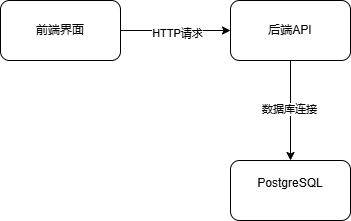
\includegraphics[width=0.8\textwidth]{pic/sap.png}  % 设置图片宽度为文档宽度的一半
    \caption{系统结构图}  % 图片标题
    \label{fig:sap}  % 图片标签,便于引用
\end{figure}

车辆租赁管理系统采用分层架构设计,
主要分为表现层、业务逻辑层和数据访问层,各层次的功能和作用如下:

\begin{itemize}
    \item 表现层(前端):\\
    表现层是系统与用户交互的部分,负责用户界面的显示和操作处理,
    包括车辆信息的查询、客户信息录入、租赁信息的修改等功能。
    具体技术采用HTML、CSS等前端技术,确保界面美观和用户体验友好。
    \item 业务逻辑层(后端):\\
    业务逻辑层位于表现层与数据访问层之间,
    是系统功能实现的核心部分,主要负责接收前端请求、
    处理业务逻辑并与数据库交互。车辆管理、租赁管理和客户管理的功能均在该层实现。
    本系统采用Django框架开发业务逻辑层,
    支持高效的请求响应和模块化开发。
    
    \item 数据访问层(数据库):\\
    数据访问层是系统的数据存储和管理部分,负责与数据库交互,
    执行SQL查询操作以实现数据的增删改查。
    本系统选用PostgreSQL作为数据库管理系统,
    设计了满足第三范式(3NF)的数据库结构,确保数据存储的规范性和完整性。
\end{itemize}

各层通过接口进行数据交互:表现层将用户请求发送给业务逻辑层,
业务逻辑层根据功能需求调用数据访问层与数据库交互,
最终返回结果至表现层供用户查看和操作。
这种分层设计提升了系统的可维护性和扩展性。

针对需求分析,我们得到了系统结构图,如图\ref{fig:sap}所示。

\subsection{系统功能模块}

\begin{figure}[htbp]  % figure 环境用于插入图片并进行浮动
    \centering  % 图片居中
    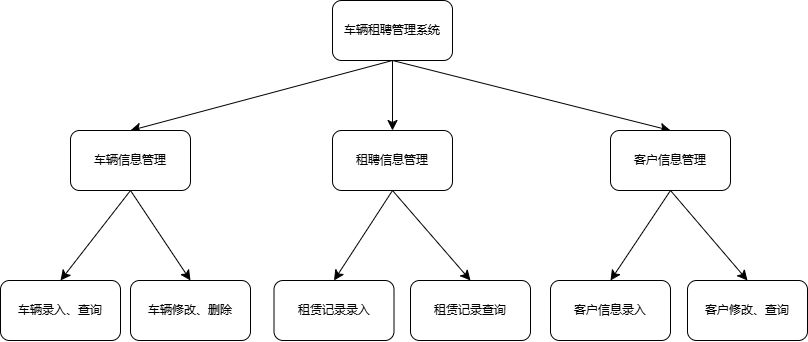
\includegraphics[width=0.8\textwidth]{pic/system_function_modules.png}  % 设置图片宽度为文档宽度的一半
    \caption{系统功能模块图}  % 图片标题
    \label{fig:sfm}  % 图片标签,便于引用
\end{figure}

车辆租赁管理系统的功能模块图以系统需求为基础,分为三个主要功能模块:
车辆信息管理模块、
租赁管理模块和客户信息管理模块。各模块的功能和相互关系描述如下:

% \vspace{-0.3cm}
\begin{itemize}
    \item 车辆信息管理模块:实现车辆信息的添加、修改等功能。\\
    添加功能用于录入车辆基本信息,如车辆编号、车型、租赁价格等。\\
    修改功能用于更新车辆状态或属性,如车辆的租赁状态、等。
    \item 租赁管理模块:实现租赁交易的管理,包括租赁信息的录入、修改和查询。\\
    录入功能记录租赁交易信息,如租赁车辆、客户、起始日期、结束日期及费用等。\\
    修改功能允许调整租赁的相关信息,如租赁时间或费用的变更。\\
    查询功能支持客户查找租赁记录,方便查看历史交易。
    \item 客户信息管理模块:实现客户信息的管理,包括添加、修改和查询功能。\\
    添加功能用于录入新客户的信息,如姓名、联系方式、身份证号等。\\
    修改功能用于更新客户信息,如更改联系方式或地址。\\
    查询功能支持按客户姓名或其他条件检索客户信息,便于用户管理客户数据。\\
\end{itemize}
\vspace{-0.8cm}
针对需求分析,我们得到了系统的功能模块图,如图\ref{fig:sfm}所示。

\section{详细设计}

\subsection{E-R图}

\begin{figure}[htbp]  % figure 环境用于插入图片并进行浮动
    \centering  % 图片居中
    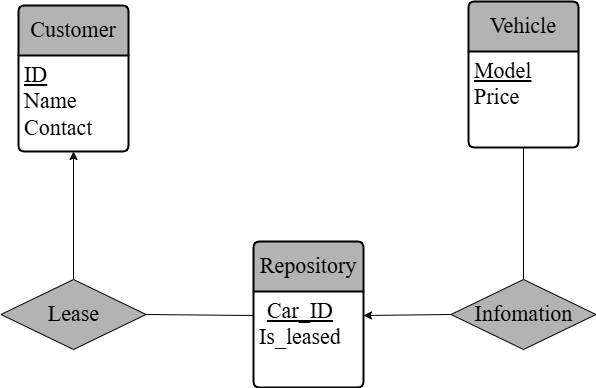
\includegraphics[width=0.8\textwidth]{pic/er.png}  % 设置图片宽度为文档宽度的一半
    \caption{E-R图}  % 图片标题
    \label{fig:er}  % 图片标签,便于引用
\end{figure}

车辆租赁管理系统的E-R图描述了系统中的主要实体及其之间的关系,
反映了系统的数据结构和逻辑关系~\cite{silberschatz2011database}。根据系统需求分析,设计了以下实体及其属性:

\subsubsection{实体及属性}

\begin{itemize}[leftmargin=0.3cm]
% \begin{itemize}
    \item 客户(Customer)属性:\\
    用户(User):与Django的内置用户模型进行一对一关联,扩展用户信息。\\
    ID(主键):客户唯一标识符。\\
    姓名(name):客户姓名。\\
    联系方式(contact):客户的联系方式。\\
\vspace{-0.7cm}
    \item 车辆(Vehicle)属性:\\
    型号(Model,主键):车辆的唯一标识。\\
    价格(Price):车辆的租赁价格。\\

    \item 车辆库(Repository)属性:\\
    车辆ID(Car\_ID,主键):标识库中每辆车的唯一编号。\\
    是否租赁(Is\_leased):表示车辆是否已被租赁。\\
\vspace{-0.7cm}
    \item 车辆信息(Info)属性:\\
    车辆ID(Car\_ID,外键):引用车辆库中的车辆ID。\\
    型号(Model,外键):引用车辆表中的型号信息。\\
\vspace{-0.7cm}    
    \item 租赁记录(Lease)属性:\\
    车辆ID(Car\_ID,外键):关联车辆库中的车辆。\\
    客户ID(ID,外键):关联客户表中的客户。\\
\end{itemize}

\subsubsection{实体之间的关系} 
\begin{itemize}[leftmargin=0.3cm]
\item 客户与租赁记录:
一个客户可以进行多次租赁记录(一对多)。

\item 车辆与车辆库:
车辆库中的每辆车属于一个车辆型号(多对一)。

\item 车辆库与租赁记录:
每辆车在租赁记录中最多出现一次(一对一)。

\item 车辆库与车辆信息:
每辆车在车辆信息表中有对应的详细记录(一对一)。
\end{itemize}
针对需求分析,画出E-R图表示的概念模型,如图\ref{fig:er}所示。

\subsection{数据库模式}

首先我们这个关系模型是满足3NF的,即第三范式。具体满足了一下条件:

\textbf{满足第一范式(1NF)}

\begin{itemize}
    \item 所有字段的值都是原子值,没有重复的组或数组。比如,\texttt{Customer} 类中的字段 \texttt{name} 和 \texttt{contact} 都是单一值,没有包含集合或数组。
    \item 每一列的值都是不可分割的。
\end{itemize}

\textbf{满足第二范式(2NF)}

\begin{itemize}
    \item 在满足第一范式的基础上,所有非主键属性完全依赖于主键。
    \item 例如,\texttt{Customer} 类中的 \texttt{name} 和 \texttt{contact} 完全依赖于主键 \texttt{ID}。这个表中的每个字段都与主键 \texttt{ID} 相关,而不是仅仅部分依赖。
    \item 在 \texttt{Lease} 类中,\texttt{Car\_ID} 和 \texttt{ID} 外键的组合确保了每条记录唯一地标识了一个租赁。 \texttt{ID} 外键依赖于 \texttt{Customer} 的 \texttt{ID},而 \texttt{Car\_ID} 外键依赖于 \texttt{Repository} 的 \texttt{Car\_ID}。
\end{itemize}

\textbf{满足第三范式(3NF)}

\begin{itemize}
    \item 除了满足第二范式外,还要求所有非主键字段必须直接依赖于主键,而不能依赖于其他非主键字段。
    \item 在 \texttt{Vehicle} 类中,字段 \texttt{Model} 是唯一标识一个车辆类型的字段,字段 \texttt{Price} 完全依赖于 \texttt{Model}。所以,\texttt{Vehicle} 表中的每个字段直接依赖于主键 \texttt{Model}。
    \item \texttt{Repository} 类中的 \texttt{Car\_ID} 是主键,并且字段 \texttt{Is\_leased} 完全依赖于主键 \texttt{Car\_ID},没有任何传递依赖。
    \item \texttt{Info} 类通过外键将 \texttt{Car\_ID} 和 \texttt{Model} 与 \texttt{Repository} 和 \texttt{Vehicle} 表关联。 \texttt{Car\_ID} 和 \texttt{Model} 作为外键,确保了数据表之间的关联关系符合规范。
    \item 在 \texttt{Lease} 类中,\texttt{Car\_ID} 和 \texttt{ID} 外键分别引用了 \texttt{Repository} 和 \texttt{Customer} 表,确保了租赁关系的唯一性,而不会引入冗余数据。
\end{itemize}

\textbf{具体范式分析}

\begin{itemize}
    \item \textbf{Customer}:
    \begin{itemize}
        \item 主键:\texttt{ID},所有字段(\texttt{name} 和 \texttt{contact})直接依赖于主键,符合第二范式。
        \item 该表没有任何字段间的传递依赖,符合第三范式。
    \end{itemize}
    
    \item \textbf{Vehicle}:
    \begin{itemize}
        \item 主键:\texttt{Model},字段 \texttt{Price} 完全依赖于 \texttt{Model},没有传递依赖,符合第二范式和第三范式。
    \end{itemize}
    
    \item \textbf{Repository}:
    \begin{itemize}
        \item 主键:\texttt{Car\_ID},字段 \texttt{Is\_leased} 完全依赖于 \texttt{Car\_ID},符合第二范式和第三范式。
    \end{itemize}
    
    \item \textbf{Info}:
    \begin{itemize}
        \item 外键 \texttt{Car\_ID} 引用 \texttt{Repository} 表,外键 \texttt{Model} 引用 \texttt{Vehicle} 表。所有字段依赖于外键,不存在传递依赖,符合第三范式。
    \end{itemize}
    
    \item \textbf{Lease}:
    \begin{itemize}
        \item 外键 \texttt{Car\_ID} 引用 \texttt{Repository},外键 \texttt{ID} 引用 \texttt{Customer}。这些字段是唯一标识租赁记录的,因此不会引入冗余数据,符合第三范式。
    \end{itemize}
\end{itemize}


该设计通过外键建立了表与表之间的关系,
并且每个表中的字段都直接依赖于主键,
避免了冗余数据,符合第三范式的要求。




根据车辆租赁管理系统的需求和 E-R 图,
将概念模型转换为关系模型,设计出满足第三范式(上面已经给予证明)的数据库模式。
具体如下:

\subsubsection{表设计}


\begin{table}[h!]
    \centering
    \caption{客户表(Customer)}
\begin{tabular}{|l|l|l|l|}
\hline
字段名 & 数据类型 & 约束 & 说明 \\
\hline
ID & VARCHAR(10) & PRIMARY KEY & 客户唯一标识符 \\
\hline
user\_id & INTEGER & UNIQUE, NOT NULL & 关联 Django 用户表 \\
\hline
name & VARCHAR(50) & NOT NULL & 客户姓名 \\
\hline
contact & VARCHAR(15) & NOT NULL & 客户联系方式 \\
\hline
\end{tabular}
\end{table}


\begin{table}[h!]
    \centering
    \caption{车辆表(Vehicle)}
\begin{tabular}{|l|l|l|l|}
\hline
字段名 & 数据类型 & 约束 & 说明 \\
\hline
Model & VARCHAR(50) & PRIMARY KEY & 车辆型号 \\
\hline
Price & INTEGER & NOT NULL & 租赁价格 \\
\hline
\end{tabular}
\end{table}


\begin{table}[h!]
    \centering
    \caption{车辆库表(Repository)}
\begin{tabular}{|l|l|l|l|}
\hline
字段名 & 数据类型 & 约束 & 说明 \\
\hline
Car\_ID & VARCHAR(10) & PRIMARY KEY & 车辆唯一标识符 \\
\hline
Is\_leased & BOOLEAN & DEFAULT FALSE & 是否被租赁 \\
\hline
\end{tabular}
\end{table}


\begin{table}[h!]
    \centering
    \caption{车辆信息表(Info)}
\begin{tabular}{|l|l|l|l|}
\hline
字段名 & 数据类型 & 约束 & 说明 \\
\hline
Car\_ID & VARCHAR(10) & FOREIGN KEY (Repository.Car\_ID), NOT NULL & 关联车辆库表 \\
\hline
Model & VARCHAR(50) & FOREIGN KEY (Vehicle.Model), NOT NULL & 关联车辆型号 \\
\hline
\end{tabular}
\end{table}


\begin{table}[h!]
    \centering
    \caption{租赁记录表(Lease)}
\begin{tabular}{|l|l|l|l|}
\hline
字段名 & 数据类型 & 约束 & 说明 \\
\hline
ID & VARCHAR(10) & FOREIGN KEY (Customer.ID), NOT NULL & 关联客户表 \\
\hline
Car\_ID & VARCHAR(10) & FOREIGN KEY (Repository.Car\_ID), NOT NULL & 关联车辆库表 \\
\hline
\end{tabular}
\end{table}

\subsubsection{数据库模式特点}

\begin{enumerate}
    \item \textbf{满足第三范式(3NF)}
    \begin{itemize}
        \item 消除冗余:每个表只存储一种实体的属性,避免数据冗余。
        \item 数据依赖明确:所有非主键字段完全依赖于主键。
    \end{itemize}
    \item \textbf{完整性约束}
    \begin{itemize}
        \item 主键约束:每个表都有明确的主键,保证数据唯一性。
        \item 外键约束:通过外键建立表间关系,保证数据一致性。
    \end{itemize}
    \item \textbf{扩展性}
    \begin{itemize}
        \item 模块化表设计便于功能扩展,如增加车辆维修管理、客户等级管理等功能。
    \end{itemize}
\end{enumerate}

% \subsection{主要功能模块设计与开发}

\subsection{车辆信息管理模块设计与开发}
车辆信息管理模块需要维护数据中的所有车辆,同时还需要提供良好的交互界面,便于用户使用和了解车辆信息。
对此,该模块的前端设计需要提供方便客户查询车辆信息和租赁的交互界面,而后端则需要维护车辆的信息。该模块的总体设计如图~\ref{fig:carman}所示,
\begin{figure}[htbp]  % figure 环境用于插入图片并进行浮动
    \centering  % 图片居中
    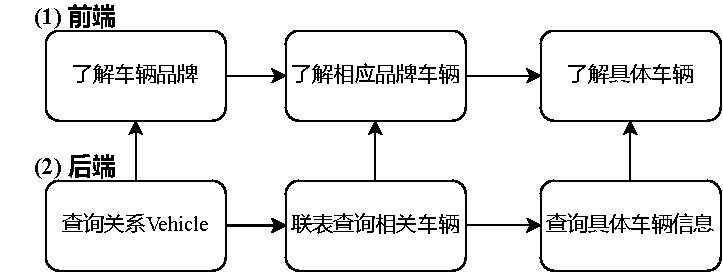
\includegraphics[width=0.8\textwidth]{pic/carman.pdf}
    \caption{车辆信息管理模块图}  % 图片标题
    \label{fig:carman}  % 图片标签,便于引用
\end{figure}
在前端,用户可以方便地查看仓库中车辆的品牌,在了解相应的车品牌后,可以查看该品牌相关的车辆并了解车辆的信息。而后端则需要对用户的行为做出合理的反应,即使反馈用户所查看的信息。

\subsubsection{实现流程}
当用户进入交互页面后,用户可以在侧边栏点击租车键,然后租车键下会展开车辆品牌信息,供用户查看。这些展开的车辆品牌也是可交互的,用户可以点击感兴趣的品牌进一步查看相应品牌的车辆有哪些,然后查看车辆的具体信息。
而用户的一系列点击行为,在后端会引发相应的数据库查询。

\subsubsection{主要算法}
实现这一模块的核心思想在于,通过用户点击 HTML 页面中的相关按钮,触发相应的 JavaScript 操作,而 JavaScript 函数进一步通过指定的 URL 调用后端服务以执行相应的查询逻辑。

在HTML文件中,添加一个租车标签,并设置onclick属性,用来指定点击该元素时要执行的JavaScript函数fetchVehicles(event),通过该函数动态填充车辆品牌列表。
\begin{lstlisting}[language=HTML]
<li>
    <a href="#" onclick="fetchVehicles(event)">租车</a>
    <ul id="vehicle-list" style="padding-left: 20px; display: none;"> </ul>
</li>
\end{lstlisting}

编写相关的JavaScript函数fetchVehicles(event)查询相应的车辆品牌。在函数中,我们通过URL连接后端端口得到车辆品牌,然后再函数中填充车辆品牌列表。
\begin{lstlisting}[language=JavaScript]
function fetchVehicles(event) {
    event.preventDefault();
    fetch('/management/get-vehicles/')
        .then(response => response.json())
        .then(data => {
            const vehicleList = document.getElementById('vehicle-list');
            vehicleList.innerHTML = ''; 

            if (data.status === "success") {
                let html = '';
                data.data.forEach(vehicle => {
                    html += `<li>
                                <a href="#" onclick="fetchVehicleDetails('${vehicle.Model}')">
                                    ${vehicle.Model}
                                </a>
                            </li>`;
                });
                vehicleList.innerHTML = html;
                vehicleList.style.display = 'block'; // 显示车辆列表
            } else {
                vehicleList.innerHTML = '<li>暂无车辆信息</li>';
                vehicleList.style.display = 'block';
            }
        })
        .catch(error => {
            console.error("Error fetching vehicles:", error);
        });
}
\end{lstlisting}

在后端views.py中编写该函数对应的相关行为,即select Model from Vehicle并返回给前端。
\begin{lstlisting}[language=Python]
def get_vehicles(request):
    vehicles = Vehicle.objects.all()
    if vehicles.exists():
        data = list(vehicles.values("Model"))
        return JsonResponse({"status": "success", "data": data})
    else:
        return JsonResponse({"status": "empty", "message": "暂无车辆信息"})
\end{lstlisting}

为了使用户可以根据车辆品牌了解车辆信息,我们需要将这些车辆品牌的标签设置为可跳转可查询的标签。在函数fetchVehicles中,我们在车辆品牌的标签处添加onclick行为,使其在被点击后可以反馈用户相关的车辆信息。
\begin{lstlisting}[language=HTML]
<a href="#" onclick="fetchVehicleDetails('${vehicle.Model}')">
    ${vehicle.Model}
</a>
\end{lstlisting}

在点击车辆品牌后,网页会触发JavaScript函数fetchVehicleDetails,这个函数会根据点击的车辆品牌返回相关的车辆和车辆信息。
这个函数的实现也是类似的,通过访问相关的URL然后触发后端的数据库查询然后得到相关数据。
\begin{lstlisting}[language=JavaScript]
function fetchVehicleDetails(name) {

fetch(`/management/get-vehicle-details/?name=${name}`)
    .then(response => response.json())
    .then(data => {
        const container = 
                    document.getElementById('vehicle-details');
        container.innerHTML = ''; 

        if (data.status === "success") {
            let html = '';
            data.data.forEach(item => {
                html += `
                    <tr>
                        <td>${item.Car_ID}</td>
                        <td>
                        ${item.Is_leased ? "已租赁" : "可租赁"}
                        </td>
                        <td>¥${item.Price}</td>
                        <td>
    ${item.Is_leased
        ? '<button disabled class="action-button" style="background-color: gray; cursor: not-allowed;">已租赁</button>'
        : `<button class="action-button" onclick="leaseVehicle('${item.Car_ID}', '${name}')">租赁</button>`}
                        </td>
                    </tr>
                `;
            });
            container.innerHTML = html;
        } else {
            container.innerHTML = `
                <tr>
                    <td colspan="4" style="color: red;">${data.message}</td>
                </tr>
            `;
        }
    })
    .catch(error => {
        console.error("Error fetching vehicle details:", error);
    });

}
\end{lstlisting}

在后端,后端根据点击的车辆品牌name进行数据库查询,即发生如下查询行为:
\begin{lstlisting}[language=SQL]
SELECT a.Car_ID, a.Is_leased, b.Price
FROM Repository a, Vehicle b
JOIN Info c ON b.Model = c.Model_id
WHERE a.Car_ID = c.Car_ID_id AND b.Model = name
\end{lstlisting}
而我们在views.py需要将这个查询嵌入到python函数之后,具体实现如下
\begin{lstlisting}[language=Python]
def get_vehicle_details(request):
    if request.method == "GET":
        car_name = request.GET.get("name")
        if not car_name:
            return JsonResponse({"status": "error", "message": "车辆名称不能为空"})

        query = """
            SELECT a."Car_ID", a."Is_leased", b."Price"
            FROM management_repository a, management_vehicle b
            JOIN management_info c ON b."Model" = c."Model_id"
            WHERE a."Car_ID" = c."Car_ID_id" AND b."Model" = %s
        """
        with connection.cursor() as cursor:
            cursor.execute(query, [car_name])
            rows = cursor.fetchall()

        data = [
            {"Car_ID": row[0], "Is_leased": row[1], "Price": row[2]}
            for row in rows
        ]

        if data:
            return JsonResponse({"status": "success", "data": data})
        else:
            return JsonResponse({"status": "empty", "message": "未找到车辆详情"})
\end{lstlisting}
至此,我们实现了车辆信息管理模块。

\subsection{租赁管理模块设计与开发}
租赁管理模块需要在交互界面实现租车和还车功能,这一功能需要便于客户的使用。同时,当客户进行租赁行为时,后端需要即使更新车辆租赁的状态,并将新的车辆租赁信息显示到用户交互页面。总体设计如图~\ref{fig:lease}所示,
\begin{figure}[htbp]  % figure 环境用于插入图片并进行浮动
    \centering  % 图片居中
    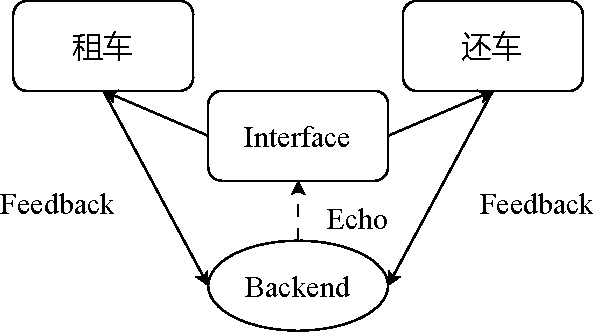
\includegraphics[width=0.8\textwidth]{pic/lease.pdf}
    \caption{用户管理模块图}  % 图片标题
    \label{fig:lease}  % 图片标签,便于引用
\end{figure}
\subsubsection{实现流程}
客户在展示车辆详细信息的页面中可以点击租车进行租车操作,然后可以在客户个人首页中点击还车按键进行还车操作。
这些客户的行为会触发后端对数据库中车辆的租赁状态进行更新并反馈到交互页面中。
\subsubsection{租车功能的算法实现}
在车辆详细信息处添加租车按键,当点击按键时会触发JavaScript函数leaseVehicle进行租车行为。同时,对于被租车辆需要禁止租车行为的发生。
\begin{lstlisting}[language=HTML]
${item.Is_leased
? '<button disabled class="action-button" style="background-color: gray; cursor: not-allowed;">已租赁</button>'
: `<button class="action-button" onclick="leaseVehicle('${item.Car_ID}', '${name}')">租赁</button>`}
\end{lstlisting}

对于函数leaseVehicle,当用户在交互页面进行租车行为触发该函数时,该函数会向租车URL提交一个表单,传递租车的客户和租赁的具体车辆。当数据库更新成功后将刷新页面,更新交互页面的信息显示。
\begin{lstlisting}[language=JavaScript]
function leaseVehicle(carId, name) {
    fetch('/management/lease-vehicle/', {
        method: 'POST',
        headers: {
            'Content-Type': 'application/json',
            'X-CSRFToken': getCookie('csrftoken') 
        },
        body: JSON.stringify({ car_id: carId })  
    })
        .then(response => response.json())
        .then(data => {
            if (data.status === "success") {
                fetchVehicleDetails(name); 
            } else {
                alert(data.message); 
            }
        })
        .catch(error => {
            console.error("Error leasing vehicle:", error);
            alert("租赁失败,请稍后再试。");
        });
}
\end{lstlisting}

在后端,当其接收到客户提交的表单时,
后端根据提交的客户信息ID和车辆信息CarID更新数据库中的关系,
即select:
\begin{lstlisting}[language=SQL]
UPDATE Repository
SET Is_leased = TRUE
WHERE Car_ID = CarID;
INSERT INTO Lease (ID,Car_ID)
VALUES (ID, CarID);
\end{lstlisting}
最后将这个SQL语句嵌入到view.py的相应处理函数中:
\begin{lstlisting}[language=Python]
@login_required
def lease_vehicle(request):
    if request.method == "POST":
        try:
            data = json.loads(request.body)
            car_id = data.get("car_id")  
            user_id = request.user.username  
            if not car_id:
                return JsonResponse({"status": "error", "message": "车辆ID不能为空"})

            update_query = """
                UPDATE management_repository
                SET "Is_leased" = TRUE
                WHERE "Car_ID" = %s
            """

            insert_query = """
                INSERT INTO management_lease ("ID_id","Car_ID_id")
                VALUES (%s, %s)
            """
            
            print(car_id)
            with connection.cursor() as cursor:
                cursor.execute(update_query, [car_id]) 
                cursor.execute(insert_query, [user_id, car_id])  
            

            return JsonResponse({"status": "success", "message": "车辆租赁成功!"})

        except Exception as e:
            print(f"Error leasing vehicle: {e}")
            return JsonResponse({"status": "error", "message": "租赁失败,请稍后再试。"})

    return JsonResponse({"status": "error", "message": "无效的请求方法"})    
\end{lstlisting}


\subsubsection{还车功能的算法实现}

系统尝试查找与当前登录用户相关联的租赁记录,查找条件包括:
车辆 ID 和用户 ID。如果没有找到匹配的租赁记录(即用户没有租过这辆车),
则抛出 Lease.DoesNotExist 异常,
并向用户显示错误信息,提示其没有租用此车辆,并将其重定向到主页。

\begin{lstlisting}[language=Python]
    try:
        lease = Lease.objects.get(Car_ID__Car_ID=vehicle_id, ID__user=request.user)
    except Lease.DoesNotExist:
        messages.error(request, "You have not rented this vehicle.")
        return redirect('homepage')
\end{lstlisting}

通过 lease 对象获取到租赁记录中关联的仓库车辆对象 Car\_ID,
然后将 Is\_leased 字段更新为 False,
表示该车辆已经被归还并且重新可用。之后调用 save() 方法保存更新。

\begin{lstlisting}[language=Python]
    repository = lease.Car_ID
    repository.Is_leased = False  # 标记车辆为未租赁
    repository.save()
\end{lstlisting}

删除租赁记录,以便用户不再与这辆车有关联,并且租赁记录从数据库中移除。

\begin{lstlisting}[language=Python]
    lease.delete()
\end{lstlisting}

\subsection{客户管理模块设计与开发}

\begin{figure}[htbp]  % figure 环境用于插入图片并进行浮动
    \centering  % 图片居中
    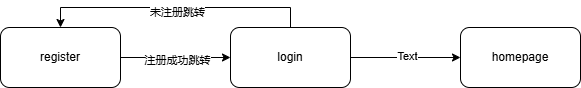
\includegraphics[width=0.8\textwidth]{pic/user_management.png}
    \caption{用户管理模块图}  % 图片标题
    \label{fig:um}  % 图片标签,便于引用
\end{figure}


总体设计如图\ref{fig:um}所示。

客户管理模块包括用户注册、登录、车辆租赁等核心功能,旨在为系统提供完整的客户管理与操作流程。

\subsubsection{用户注册功能(Register)}
注册功能实现了用户创建账户的操作,并且在创建用户时,将其信息保存到自定义的 \texttt{Customer} 表中,确保系统能够关联用户和客户之间的关系。

\textbf{实现流程}:
\begin{itemize}
    \item \textbf{GET 请求}:用户访问注册页面时,渲染 \texttt{register.html} 模板。
    \item \textbf{POST 请求}:用户提交注册表单数据时,首先进行简单校验(确保所有字段填写)。如果数据不完整或者用户名已存在,返回错误提示。
    \item 然后,使用 Django 的 \texttt{transaction.atomic()} 来保证数据的一致性,在同一个事务中创建 \texttt{User} 和 \texttt{Customer} 实例。
    \item 如果一切正常,返回成功信息并重定向到登录页面。
\end{itemize}

\textbf{主要算法}:
\begin{itemize}
    \item \textbf{字段校验}:确保用户输入的所有字段有效。
    \item \textbf{事务控制}:通过 \texttt{transaction.atomic()} 保证 \texttt{User} 和 \texttt{Customer} 的数据一致性。
    \item \textbf{异常捕获}:通过 \texttt{try-except} 结构处理注册过程中可能出现的异常,并记录日志。
\end{itemize}

\textbf{代码片段}:
\begin{lstlisting}[language=Python]
# POST 请求时
if request.method == 'POST':
    username = request.POST.get('username', '').strip()
    password = request.POST.get('password', '').strip()
    contact = request.POST.get('contact', '').strip()

    # 校验必填字段
    if not username or not password or not contact:
        messages.error(request, 'All fields are required.')
        return render(request, 'management/register.html')

    # 检查用户名是否已存在
    if User.objects.filter(username=username).exists():
        messages.error(request, 'Username already exists. Please choose another one.')
        return render(request, 'management/register.html')

    # 创建用户和客户信息
    try:
        with transaction.atomic():
            user = User.objects.create_user(username=username, password=password)
            Customer.objects.create(user=user, ID=username, name=username, contact=contact)

        messages.success(request, 'Registration successful! Please log in.')
        return redirect('login')

    except Exception as e:
        logger.error(f"Error during registration: {e}")
        messages.error(request, 'An error occurred during registration. Please try again.')
        return render(request, 'management/register.html')
\end{lstlisting}

\subsubsection{用户登录功能(Login)}
登录功能允许已注册的用户通过用户名和密码登录。系统会验证用户的凭证,
如果正确则跳转到主页homepage,否则提示登录失败。

\textbf{实现流程}:
\begin{itemize}
    \item 用户提交用户名和密码后,使用 \texttt{authenticate()} 验证其凭证。
    \item 如果验证成功,使用 \texttt{login()} 登录用户并重定向到主页。
    \item 如果验证失败,记录错误日志并返回错误信息。
\end{itemize}

\textbf{主要算法}:
\begin{itemize}
    \item \textbf{身份验证}:通过 \texttt{authenticate()} 校验用户名和密码。
    \item \textbf{登录操作}:通过 \texttt{login()} 将用户登录状态保存在会话中。
\end{itemize}

\textbf{代码片段}:
\begin{lstlisting}[language=Python]
def login_view(request):
    if request.method == 'POST':
        username = request.POST['username']
        password = request.POST['password']
        user = authenticate(request, username=username, password=password)
        if user is not None:
            login(request, user)
            logger.info(f"User {username} logged in successfully.")
            return redirect('homepage')  # 登录成功后跳转到用户仪表盘
        else:
            logger.error(f"Failed login attempt for username {username}.")
            messages.error(request, 'Invalid username or password.')
    return render(request, 'management/login.html')
\end{lstlisting}

\subsubsection{系统中的用户信息记录}

通过上述登录功能的实现,我们就可以在租车系统中的任何位置获取到当前登录的用户信息
(如用户名、联系方式等),以便于后续的租车操作和信息管理。

我们可以通过view函数中的request对象获取当前登录的用户信息,如下所示:

\begin{lstlisting}[language=Python]
    user_id = request.user.username  # 获取当前用户ID
\end{lstlisting}

因为Django 默认会将 request.user 传递到模板中,
所以我们也可以通过直接在模板中访问它,而不需要在视图中显式传递,如下所示:

\begin{lstlisting}[language=JavaScript]
    
    <p style="font-size: 24px; font-family: 'Dancing Script', cursive; color: #7b1efc; font-weight: bold;">
        Welcome, <strong>{{ user.username }}</strong>
    </p>
\end{lstlisting}

当然,如果没有登录,我们会判断出来,通过按钮跳转到login或者register页面。

\begin{lstlisting}[language=JavaScript]
    
        <p>Please log in or register to start renting vehicles.</p>
        <a href="" class="login-button">Login</a>
        <a href="" class="register-button">Register</a>
    
\end{lstlisting}

用户应该在看到自己的账号名下有什么已经租聘的车辆。
正如我们在3.4.3的还车算法中看到的,我们只需要在前端将当前用户名下的车辆渲染出来即可。

\begin{lstlisting}[language=JavaScript]
    <!-- 我的租赁部分 -->
        <div class="card-container">
            <div class="card">
                <h3 style="text-align: center;">我的租赁</h3>
                <div class="table-container">
                    <table>
                        <thead>
                            <tr>
                                <th>车牌号</th>
                                <th>车型</th>
                                <th>价格</th>
                                <th>操作</th>
                            </tr>
                        </thead>
                        <tbody>
                            
                                <tr>
                                    <td>{{ car.license_plate }}</td>
                                    <td>{{ car.model }}</td>
                                    <td>¥{{ car.price }}</td>
                                    <td>
                                        <!-- 还车按钮 -->
                                        <form action="" method="POST" style="display:inline;">
                                            
                                            <input type="hidden" name="vehicle_id" value="{{ car.license_plate }}">
                                            <button type="submit" class="btn-danger">还车</button>
                                        </form>
                                    </td>
                                </tr>
                            
                                <tr>
                                    <td colspan="4">暂无租赁车辆</td>
                                </tr>
                            
                        </tbody>
                    </table>
                </div>
            </div>
\end{lstlisting}

\subsection{安全性与完备性}


为了确保车辆租赁管理系统的数据库安全性与完备性,采取了以下设计和实现措施:

\subsubsection{用户认证与权限管理}
\begin{itemize}
    \item \textbf{用户认证}:通过 Django 内置的用户认证系统(Authentication System),对系统用户进行登录验证,确保只有授权用户能够访问系统。
    \item \textbf{权限控制}:基于角色分配权限,不同用户(如管理员和普通用户)拥有不同的数据库访问权限。例如:
    \begin{itemize}
        \item 管理员:拥有添加、修改、删除数据的权限。
        \item 普通用户:仅能查看车辆信息和提交租赁请求。
    \end{itemize}
\end{itemize}

\subsubsection{数据完整性约束}
\begin{itemize}
    \item \textbf{主键约束}:每张表都有主键,确保每条记录具有唯一标识符。
    \item \textbf{外键约束}:外键关系保证了数据的一致性,例如租赁记录表中的车辆 ID 和客户 ID 必须合法且存在。
    \item \textbf{非空约束}:关键字段(如客户姓名、联系方式等)设置为非空,确保数据完整。
    \item \textbf{默认值约束}:为布尔字段(如车辆是否租赁)设置默认值,减少人为错误。
\end{itemize}

\subsubsection{数据保护与加密}
\begin{itemize}
    \item \textbf{敏感数据加密}:对于用户的敏感信息(如密码),使用 Django 提供的密码哈希功能进行加密存储。
\end{itemize}

Django 的 User 模型已经内置了密码哈希功能,
因此只需要使用 create\_user 方法来处理用户密码。
下面是我们实现的思路:

\begin{lstlisting}[language=python]
    # 创建用户并加密密码
    user = User.objects.create_user(username=username, password=password)
\end{lstlisting}

\subsubsection{日志记录与审计}
\begin{itemize}
    \item 系统记录所有数据库操作的日志,包括数据添加、修改、删除等关键操作。
    \item 日志可用于追踪用户操作行为,及时发现和响应潜在的安全威胁。
\end{itemize}

\begin{lstlisting}[language=python]
    LOGGING = {
    'version': 1,
    'disable_existing_loggers': False,
    'formatters': {
        'verbose': {
            'format': '{levelname} {asctime} {module} {message}',
            'style': '{',
        },
        'simple': {
            'format': '{levelname} {message}',
            'style': '{',
        },
    },
    'handlers': {
        'console': {
            'level': 'DEBUG',
            'class': 'logging.StreamHandler',
            'formatter': 'simple',
        },
        'file': {
            'level': 'INFO',
            'class': 'logging.FileHandler',
            'filename': 'myapp.log',
            'formatter': 'verbose',
        },
    },
    'loggers': {
        'django': {
            'handlers': ['console'],
            'level': 'DEBUG',
            'propagate': True,
        },
        'myapp': {
            'handlers': ['console', 'file'],
            'level': 'DEBUG',
            'propagate': True,
        },
    },
}
\end{lstlisting}

在views.py中,我们可以记录用户操作日志,如下所示:

\begin{lstlisting}[language=python]
    if User.objects.filter(username=username).exists():
            logger.warning(f"Username {username} already exists.")
            messages.error(request, 'Username already exists. Please choose another one.')
            return render(request, 'management/register.html')
\end{lstlisting}

然后我们操作后就可以在myapp.log文件中看到相关日志。

\begin{lstlisting}[language=bash]
    WARNING 2024-12-25 10:36:47,223 views Username demo already exists.
    INFO 2024-12-25 10:41:41,707 views User demo logged in successfully.
    INFO 2024-12-25 10:41:43,616 views User demo returned vehicle with ID XPENG001.
    INFO 2024-12-25 10:41:54,603 views User demo returned vehicle with ID XPENG001.
\end{lstlisting}

\subsubsection{最小权限原则}
\begin{itemize}
    \item 数据库账户的权限设置遵循最小权限原则,只赋予完成任务所需的最低权限,避免权限过高导致的安全隐患。
\end{itemize}

通过以上安全性设计,系统能够有效保护数据免受未授权访问、篡改或丢失,确保数据库的完整性、保密性和可用性。

\section{调试与运行结果}
\subsection{问题与调试}


\subsubsection{\texttt{request.user} 为匿名用户}

如果用户没有登录,\texttt{request.user} 会是一个 \texttt{AnonymousUser} 实例,而不是 \texttt{User} 实例。在这种情况下,\texttt{request.user} 的属性(如 \texttt{username}、\texttt{email})可能会导致错误或不符合预期。

\paragraph{解决方法:}
\begin{itemize}
    \item 使用 \texttt{request.user.is\_authenticated} 判断用户是否登录,以避免访问匿名用户的属性。
    \item 如果用户未登录,确保有对应的处理策略。
\end{itemize}


\begin{lstlisting}[language=Python]
    user_id = request.user.username  # 获取当前用户ID
\end{lstlisting}

\subsubsection{\texttt{Customer} 模型与 \texttt{User} 模型的关系未正确配置}

在代码中,如果通过 \texttt{User} 对象来查找 \texttt{Customer} 对象时,确保 \texttt{User} 和 \texttt{Customer} 模型之间的关系正确配置(例如,\texttt{Customer} 是通过 \texttt{User} 外键关联的)。

\paragraph{解决方法:}
\begin{itemize}
    \item 确保在 \texttt{Customer} 模型中有一个外键字段指向 \texttt{User} 模型,并且关系设置正确。
\end{itemize}

\begin{lstlisting}[language=Python]
    class Customer(models.Model):
    user = models.OneToOneField(User, on_delete=models.CASCADE)
    ID = models.CharField(max_length=10, primary_key=True)  # 使用 'ID' 作为主键
    name = models.CharField(max_length=50)
    contact = models.CharField(max_length=15)

    def __str__(self):
        return self.name
\end{lstlisting}

\begin{itemize}
    \item 使用 \verb|get_object_or_404| 来获取关联的 \verb|Customer.DoesNotExist| 异常。
\end{itemize}



\begin{lstlisting}[language=Python]
from django.shortcuts import get_object_or_404  

try:
    # 获取当前登录的用户来查找关联的 Customer 实例
    customer = get_object_or_404(Customer, user=request.user)
\end{lstlisting}

\subsubsection{用户信息在模板中无法访问}

如果在模板中无法访问 \texttt{request.user} 或 \texttt{user} 变量,可能是由于模板没有正确获取上下文中的用户信息。

\paragraph{解决方法:}
\begin{itemize}
    \item 确保模板中有 if user.is\_authenticated 判断语句,并正确引用 \texttt{user} 变量。
    \item 如果自定义了中间件或修改了上下文,需要确保 \texttt{user} 被传递到模板中。
\end{itemize}

\begin{lstlisting}[language=HTML]
    <div class="user-info">
        
            <p style="font-size: 24px; font-family: 'Dancing Script', cursive; color: #7b1efc; font-weight: bold;">
                Welcome, <strong>{{ user.username }}</strong>
            </p>
        
            <p>Please log in or register to start renting vehicles.</p>
            <a href="" class="login-button">Login</a>
            <a href="" class="register-button">Register</a>
        
    </div>
\end{lstlisting}

\subsubsection{\texttt{@login\_required} 装饰器没有正确应用}

\texttt{@login\_required} 装饰器要求用户登录才能访问视图,如果没有正确应用,可能会导致未登录用户能够访问需要登录才能访问的视图。

\paragraph{解决方法:}
\begin{itemize}
    \item 确保视图函数上正确应用了 \texttt{@login\_required} 装饰器。
\end{itemize}

\begin{lstlisting}[language=Python]
from django.contrib.auth.decorators import login_required  
@login_required
def rent_car_view(request):
\end{lstlisting}

\begin{itemize}
    \item 如果 \texttt{@login\_required} 装饰器不适用,用户会被自动重定向到登录页面。可以通过设置 \texttt{LOGIN\_URL} 来修改重定向的登录页面:
\end{itemize}

\begin{lstlisting}[language=Python]
LOGIN_URL = '/management/login/'  # 登录页面
\end{lstlisting}

\subsection{最终结果展示}
经过精细的设计,我们实现了具备有注册登录功能的全面的精美的租车管理系统。在这个阶段中,我们将以用户视角展示我们的车辆租赁管理系统。
\subsubsection{注册与登录}
图~\ref{fig:reg}展示了该系统的注册页面,用户在注册页面中填入用户名,密码和邮箱,在不发生用户冲突的情况下即可注册成功。注册成功后页面会跳转到登录界面便于用户登录。由于对用户信息的保护这个过程是加密的,非明文的,所以这个过程对客户来说时安全的,无需担心的。
\begin{figure}[htbp]  % figure 环境用于插入图片并进行浮动
    \centering  % 图片居中
    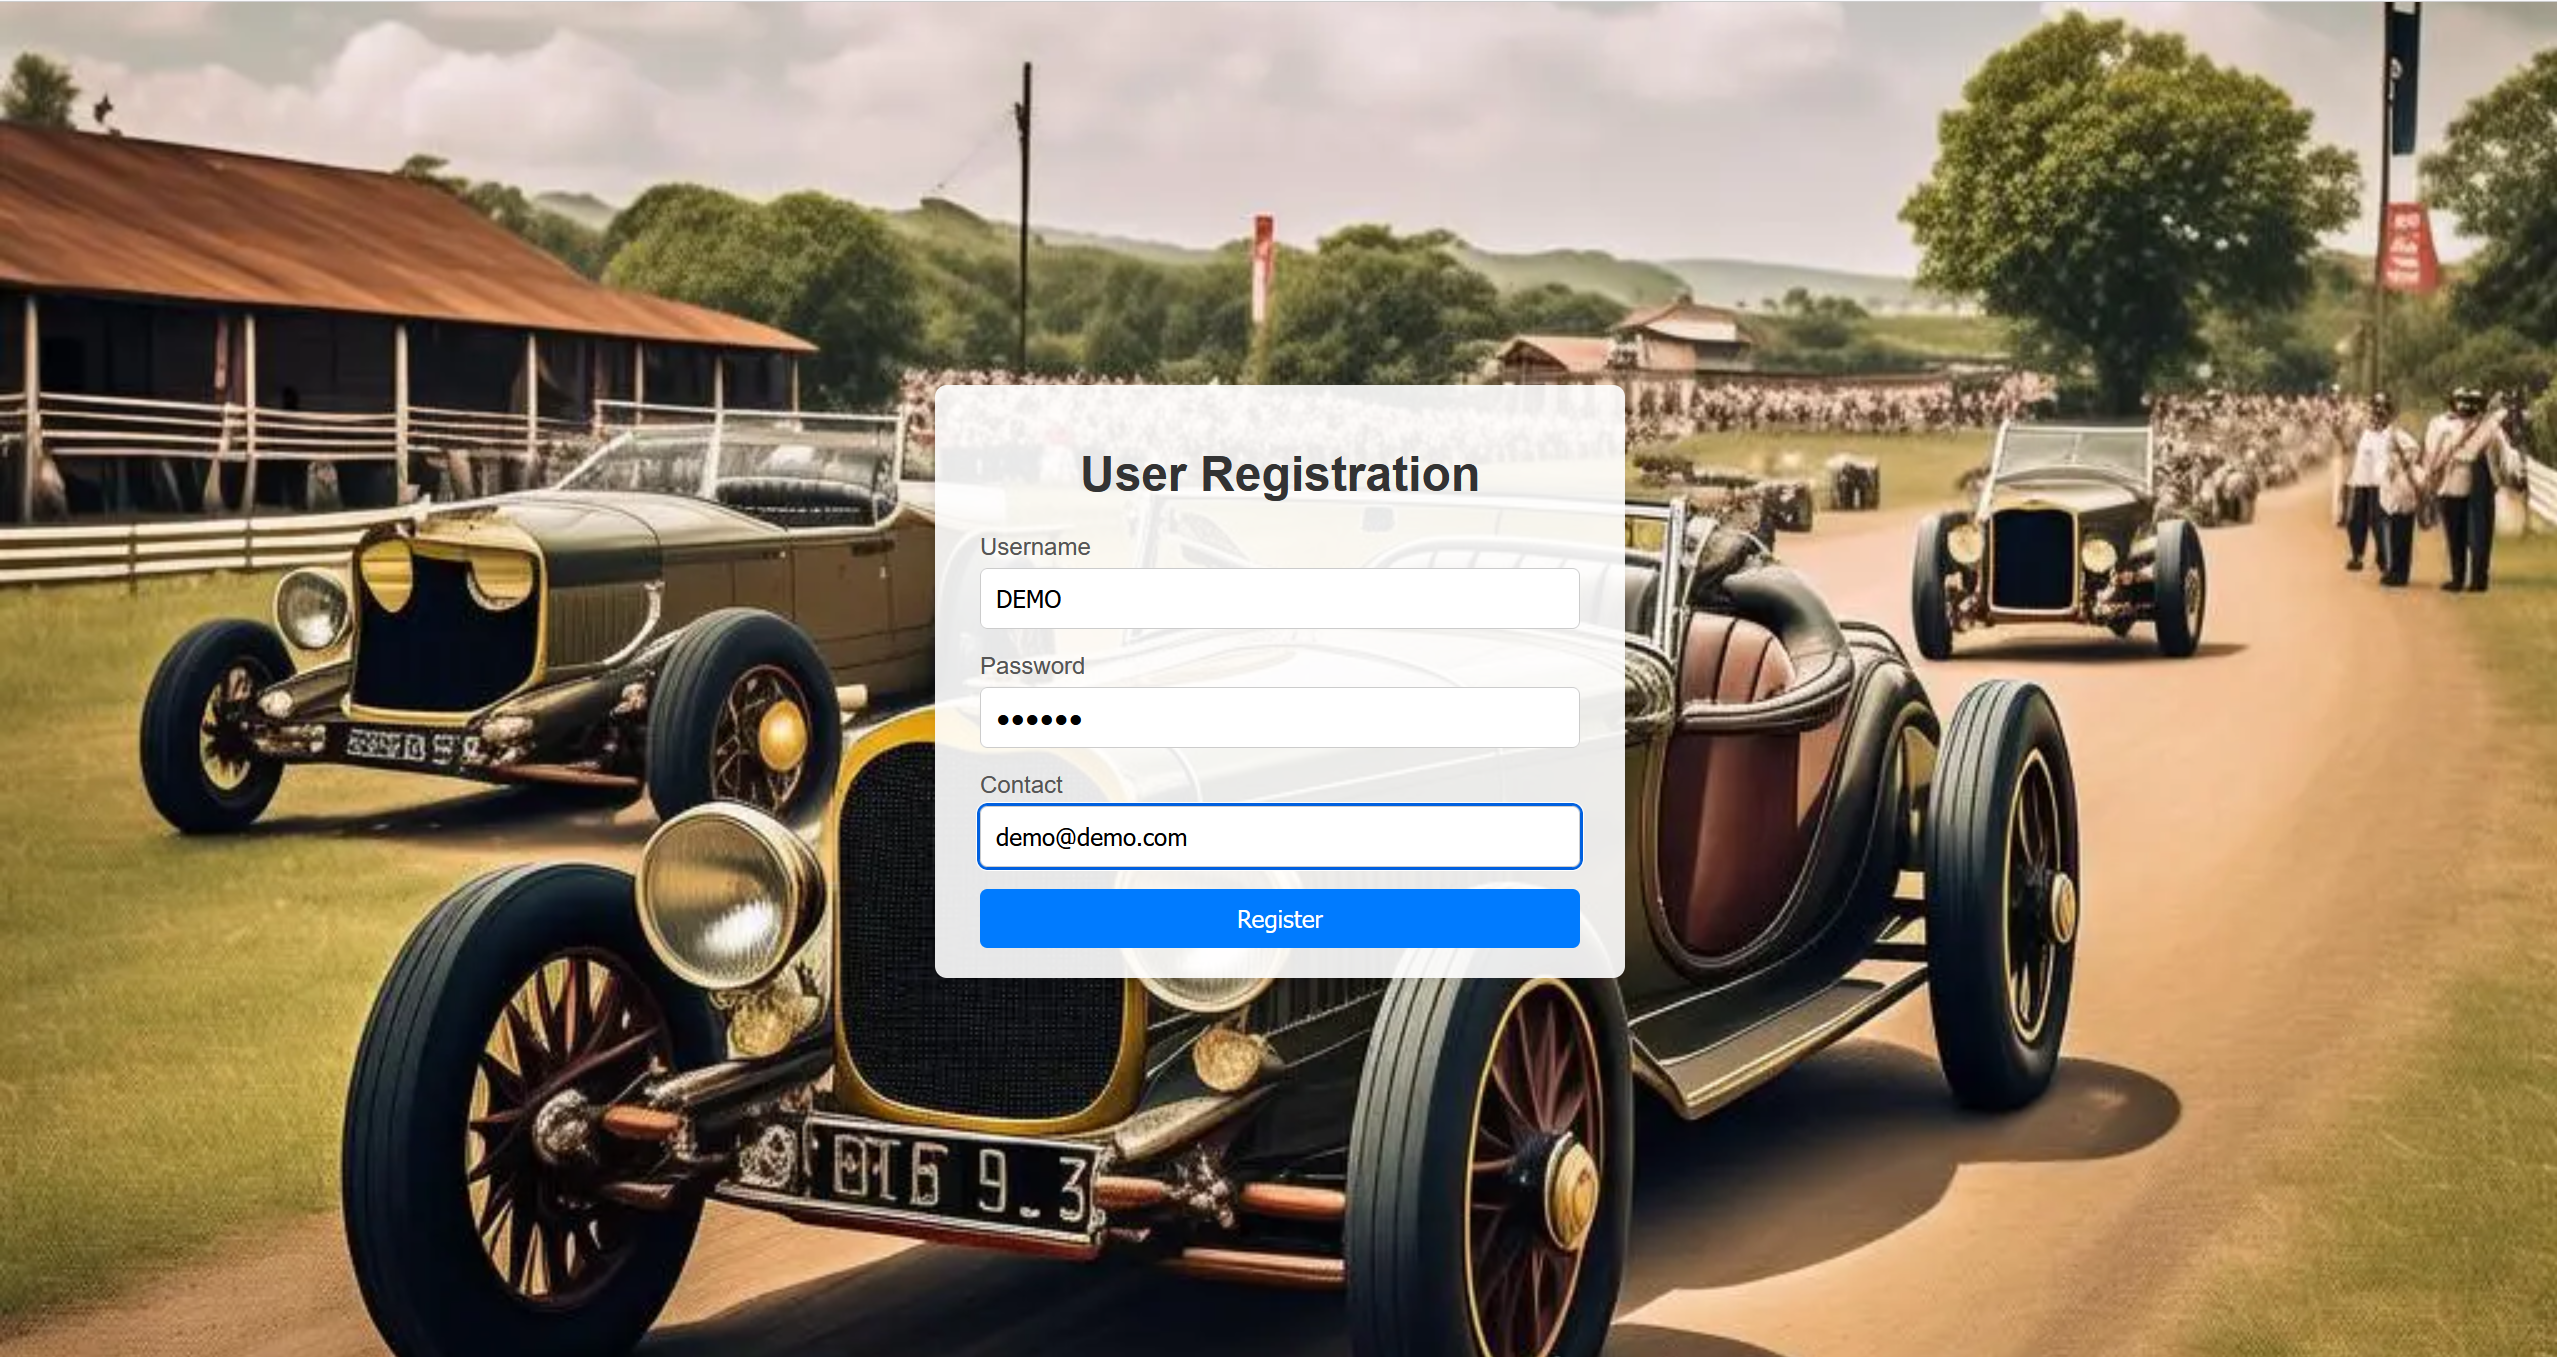
\includegraphics[width=0.8\textwidth]{pic/reg.png}
    % 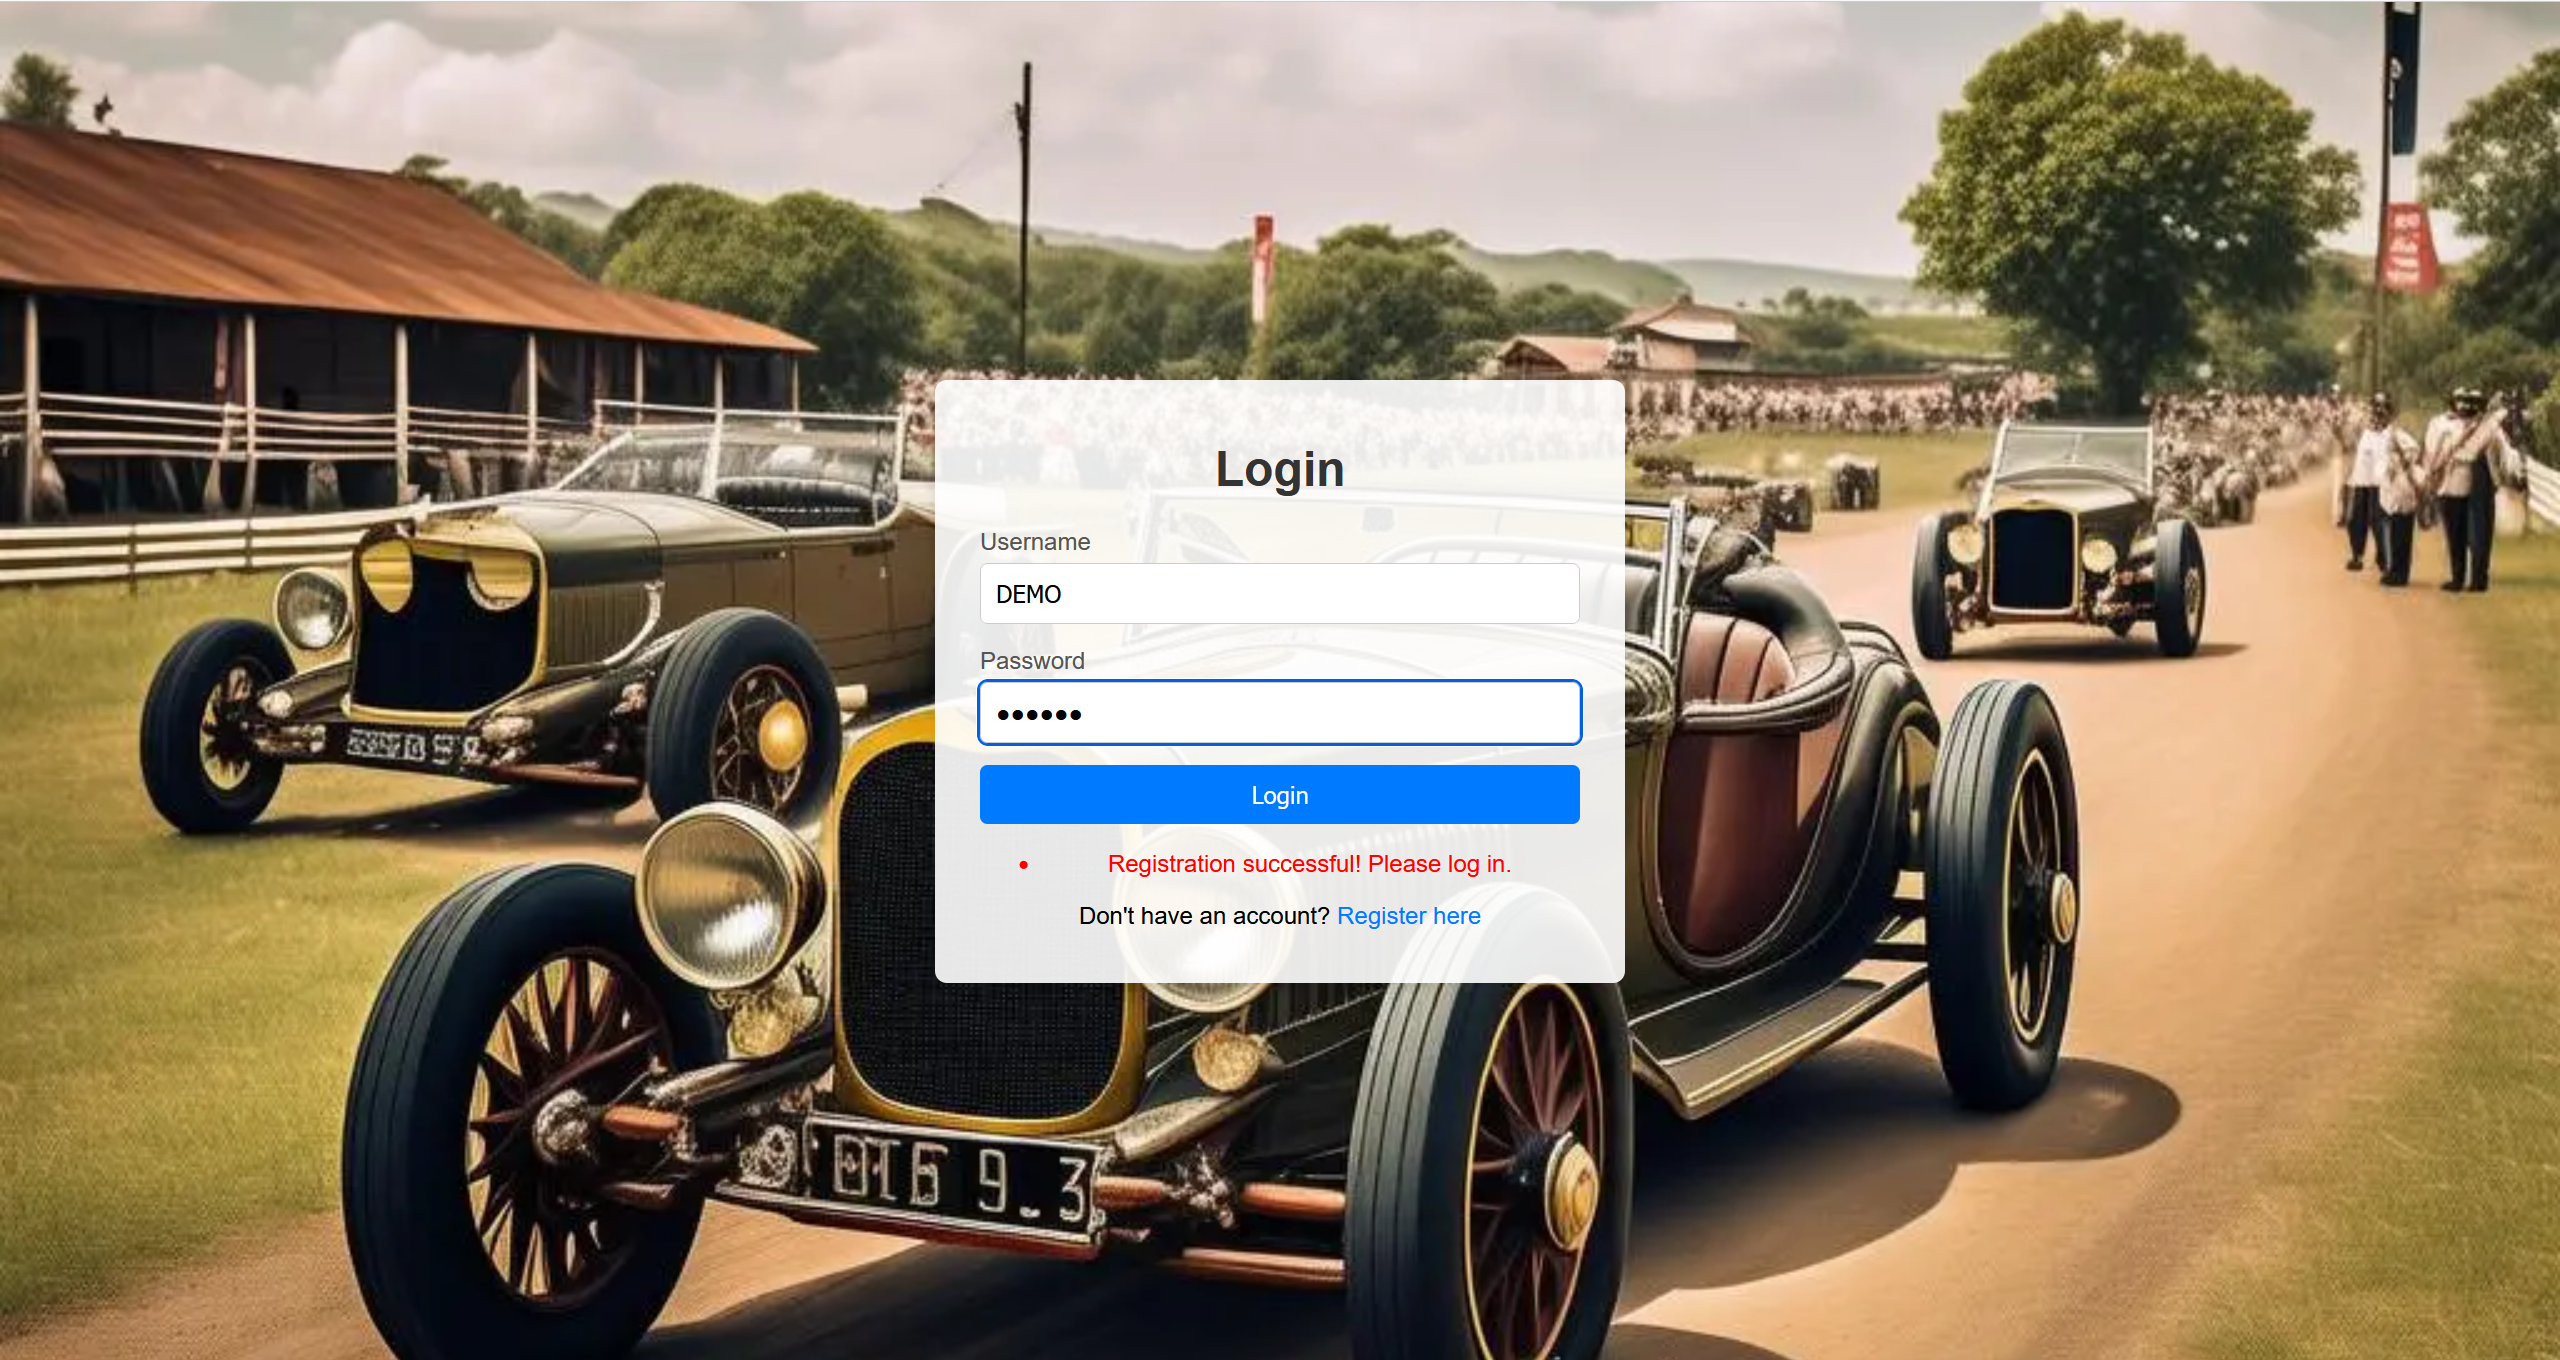
\includegraphics[width=0.8\textwidth]{pic/log.png}
    \caption{用户注册界面}  % 图片标题
    \label{fig:reg}  % 图片标签,便于引用
\end{figure}

图\ref{fig:log}展示了该系统的登录界面,用户可以主动访问该界面,或者在注册成功后跳转到该界面进行登录。用户只需填写刚才注册的用户名和密码,在信息校验成功后即登录成功,将会进入专属该用户的首页中。在登录页面,我们还加入了注册界面跳转连接,当用户发现没有账号时可以在登录页面便利地跳转到注册页面进行注册。
\begin{figure}[htbp]  % figure 环境用于插入图片并进行浮动
    \centering  % 图片居中
    % 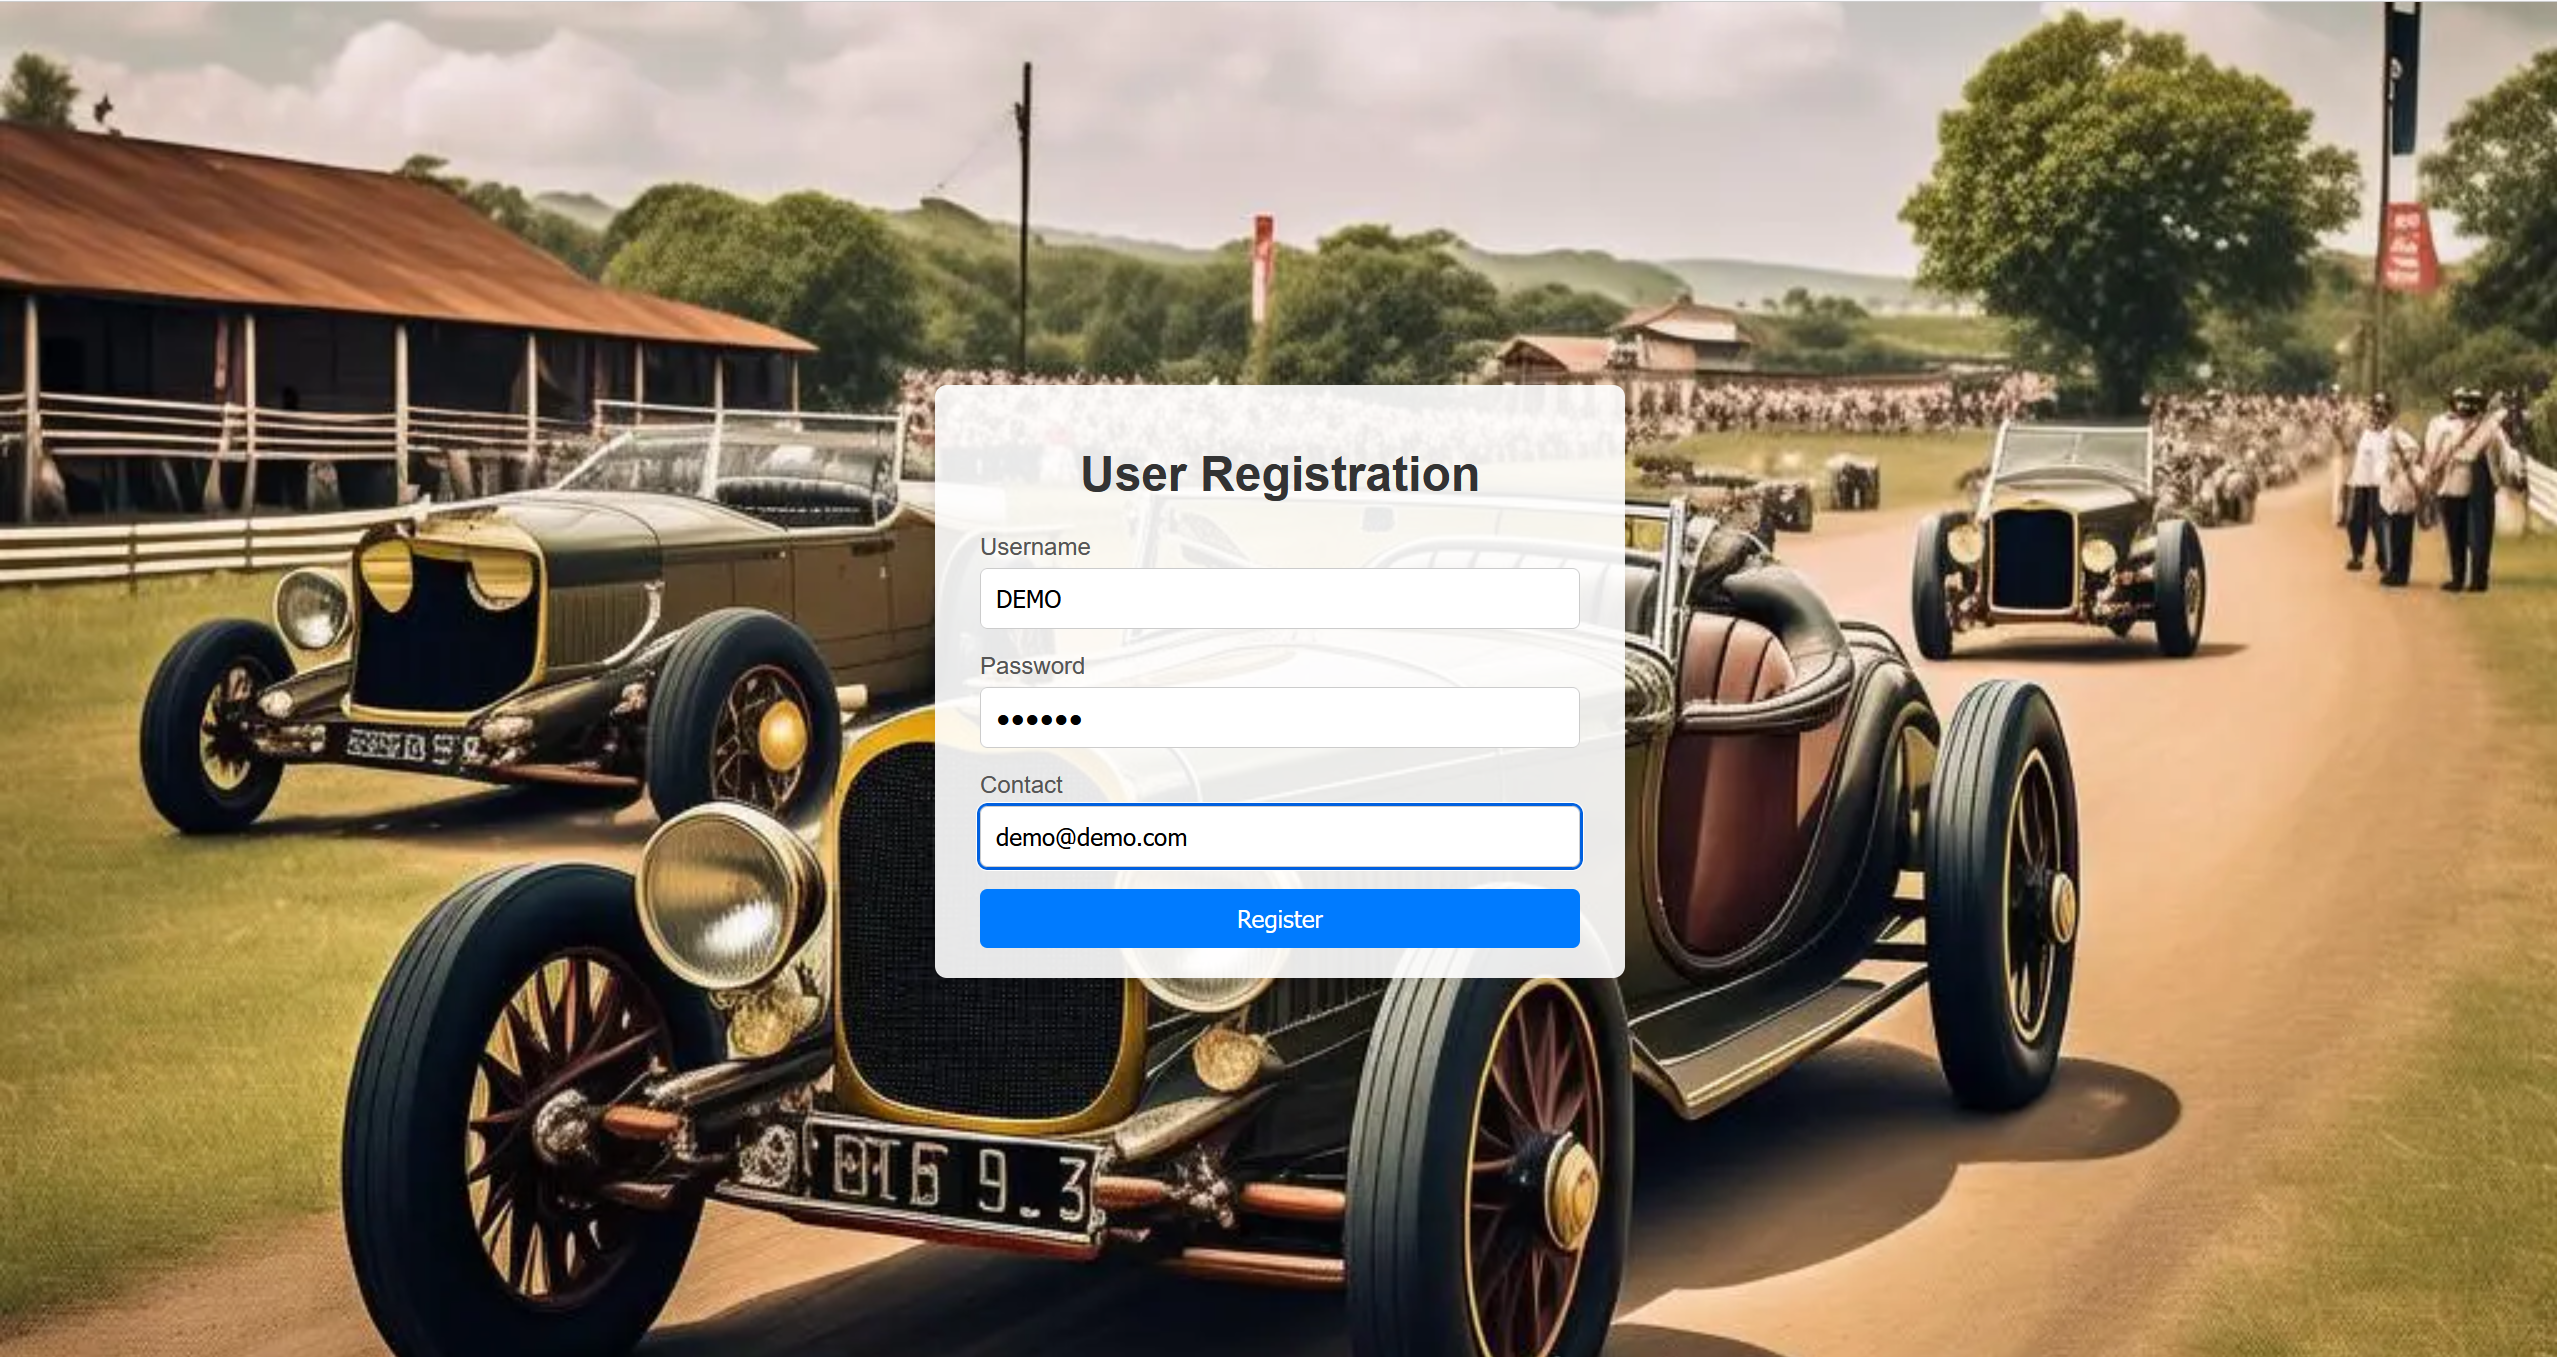
\includegraphics[width=0.8\textwidth]{pic/reg.png}
    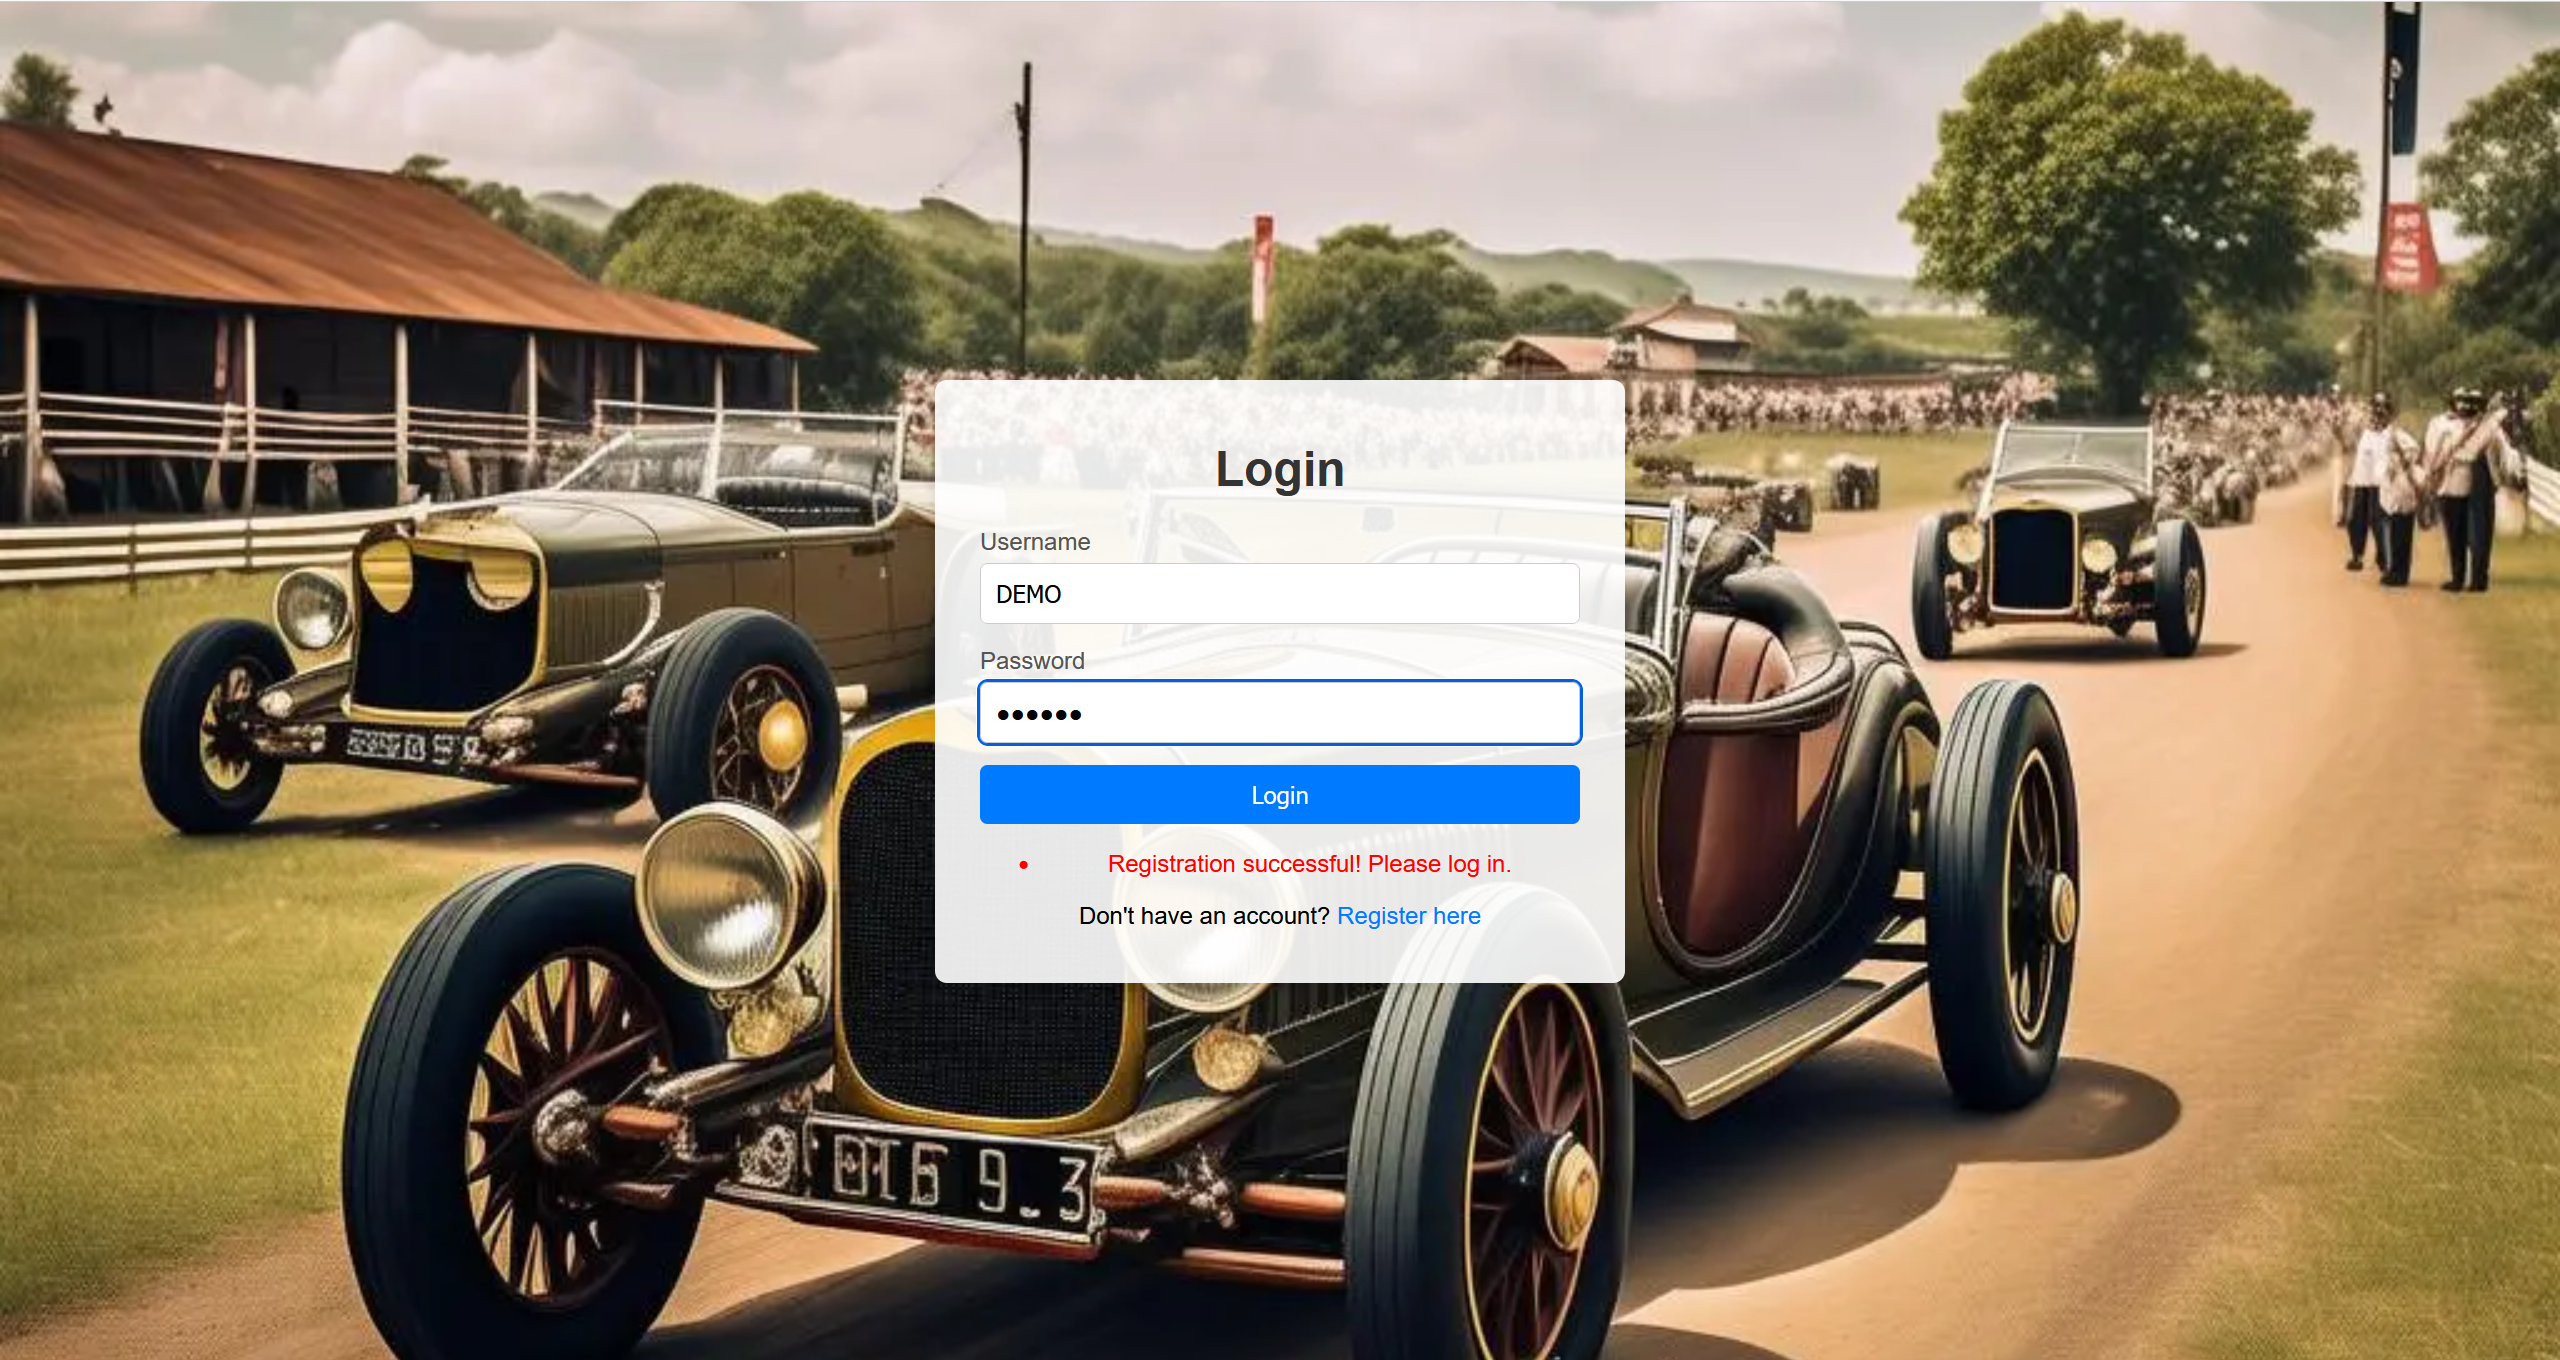
\includegraphics[width=0.8\textwidth]{pic/log.png}
    \caption{用户登录界面}  % 图片标题
    \label{fig:log}  % 图片标签,便于引用
\end{figure}

\subsubsection{用户首页}
登录成功进入用户首页后,用户可以查看自己当前的租车状态。在该侧面的侧边栏由两个按键,一个是首页,用户可以通过这个按键访问首页即图片现实的内容。另一个是租车,用户可以通过租车键查看车辆品牌,并进一步访问详细车辆信息。
\begin{figure}[htbp]  % figure 环境用于插入图片并进行浮动
    \centering  % 图片居中
    % 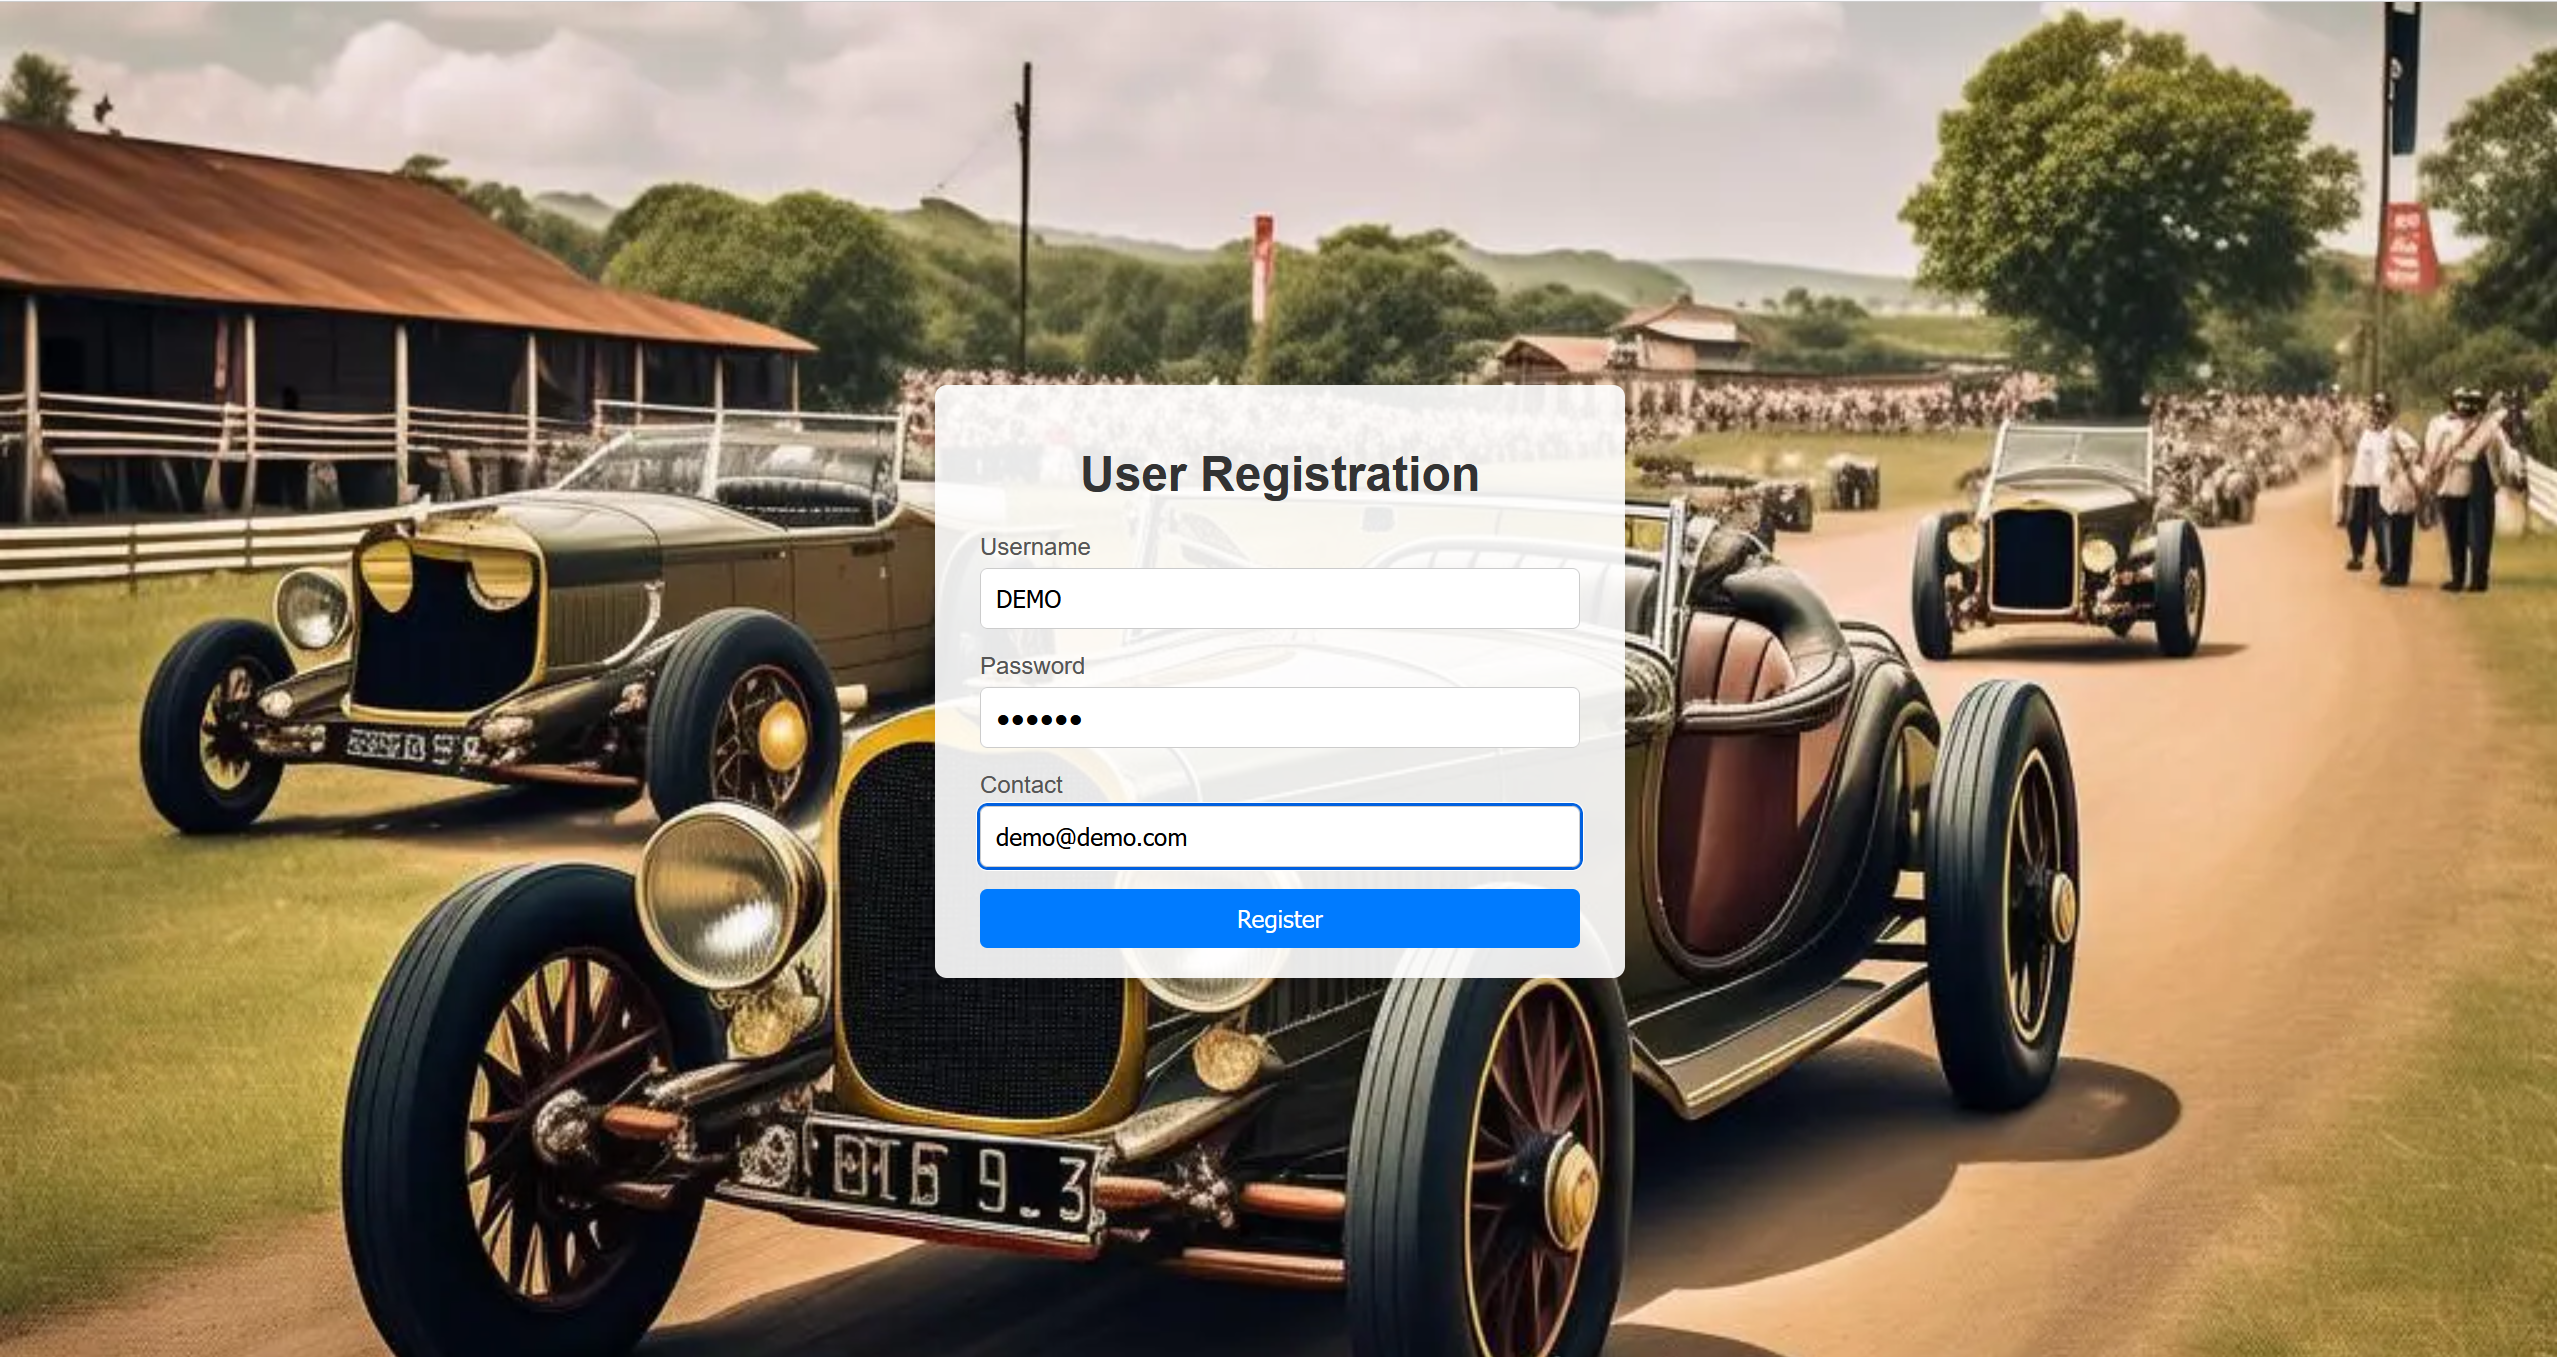
\includegraphics[width=0.8\textwidth]{pic/reg.png}
    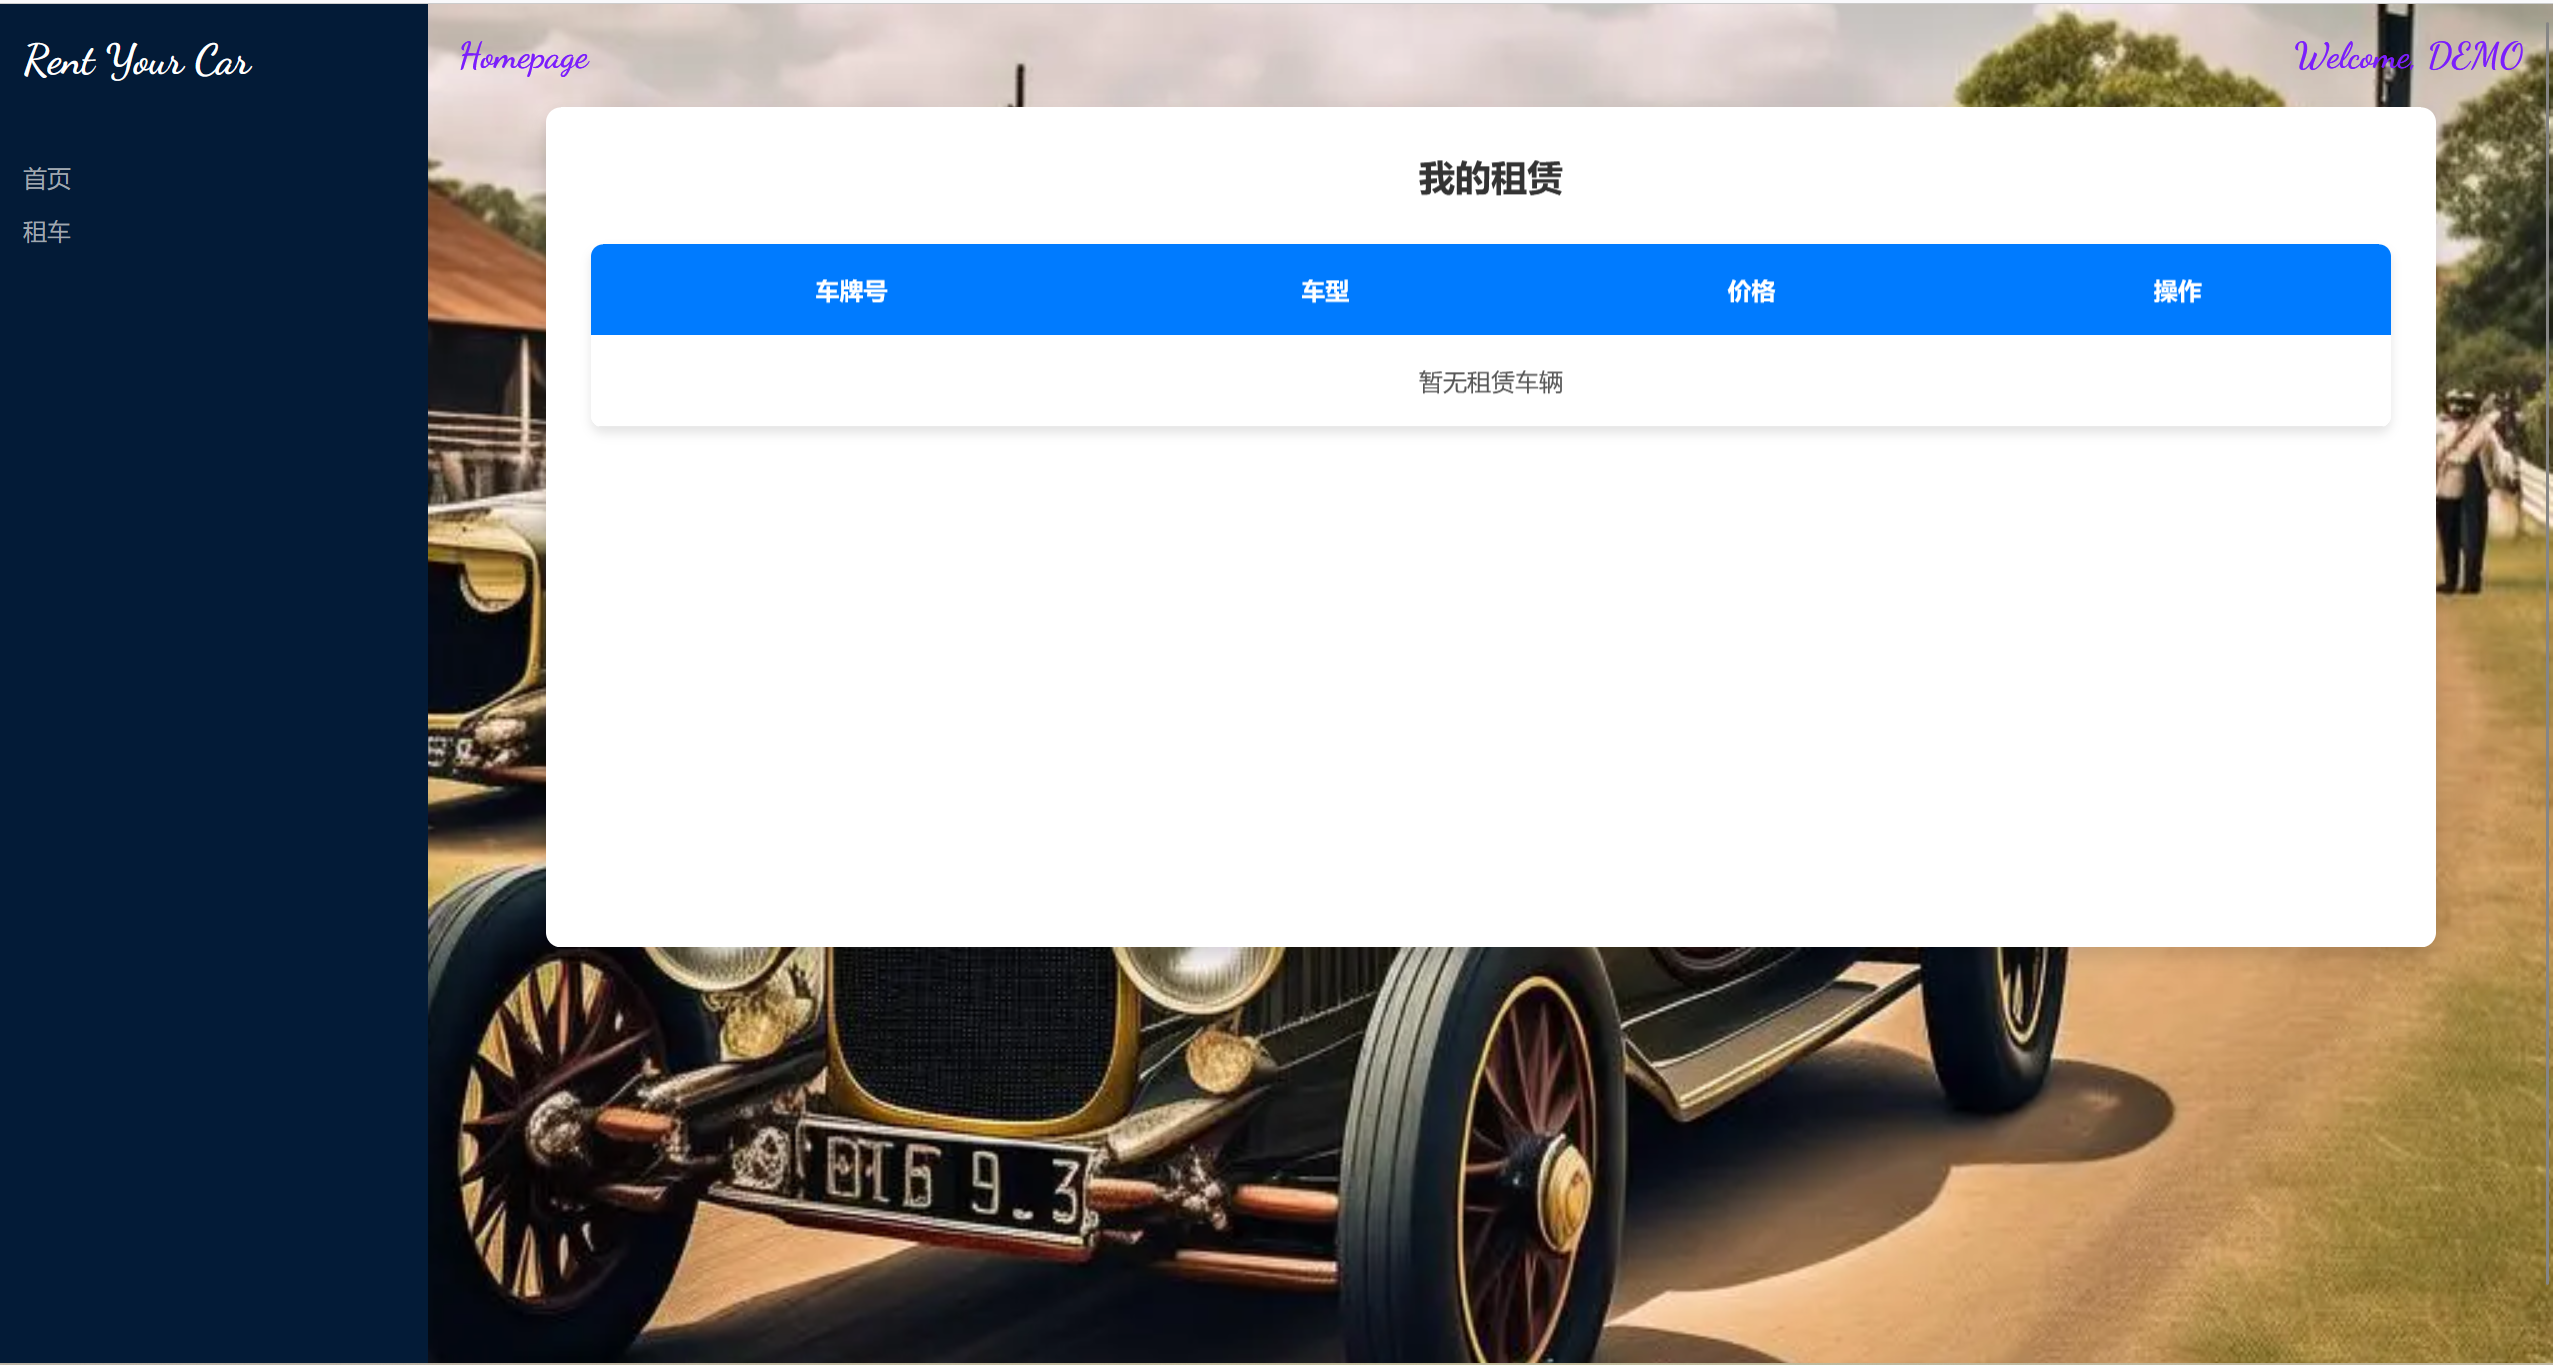
\includegraphics[width=0.8\textwidth]{pic/home.png}
    \caption{用户首页}  % 图片标题
    \label{fig:home}  % 图片标签,便于引用
\end{figure}

当用户租车后,该用户的租车信息会显示在首页中,如图~\ref{fig:rent}所示
\begin{figure}[htbp]  % figure 环境用于插入图片并进行浮动
    \centering  % 图片居中
    % 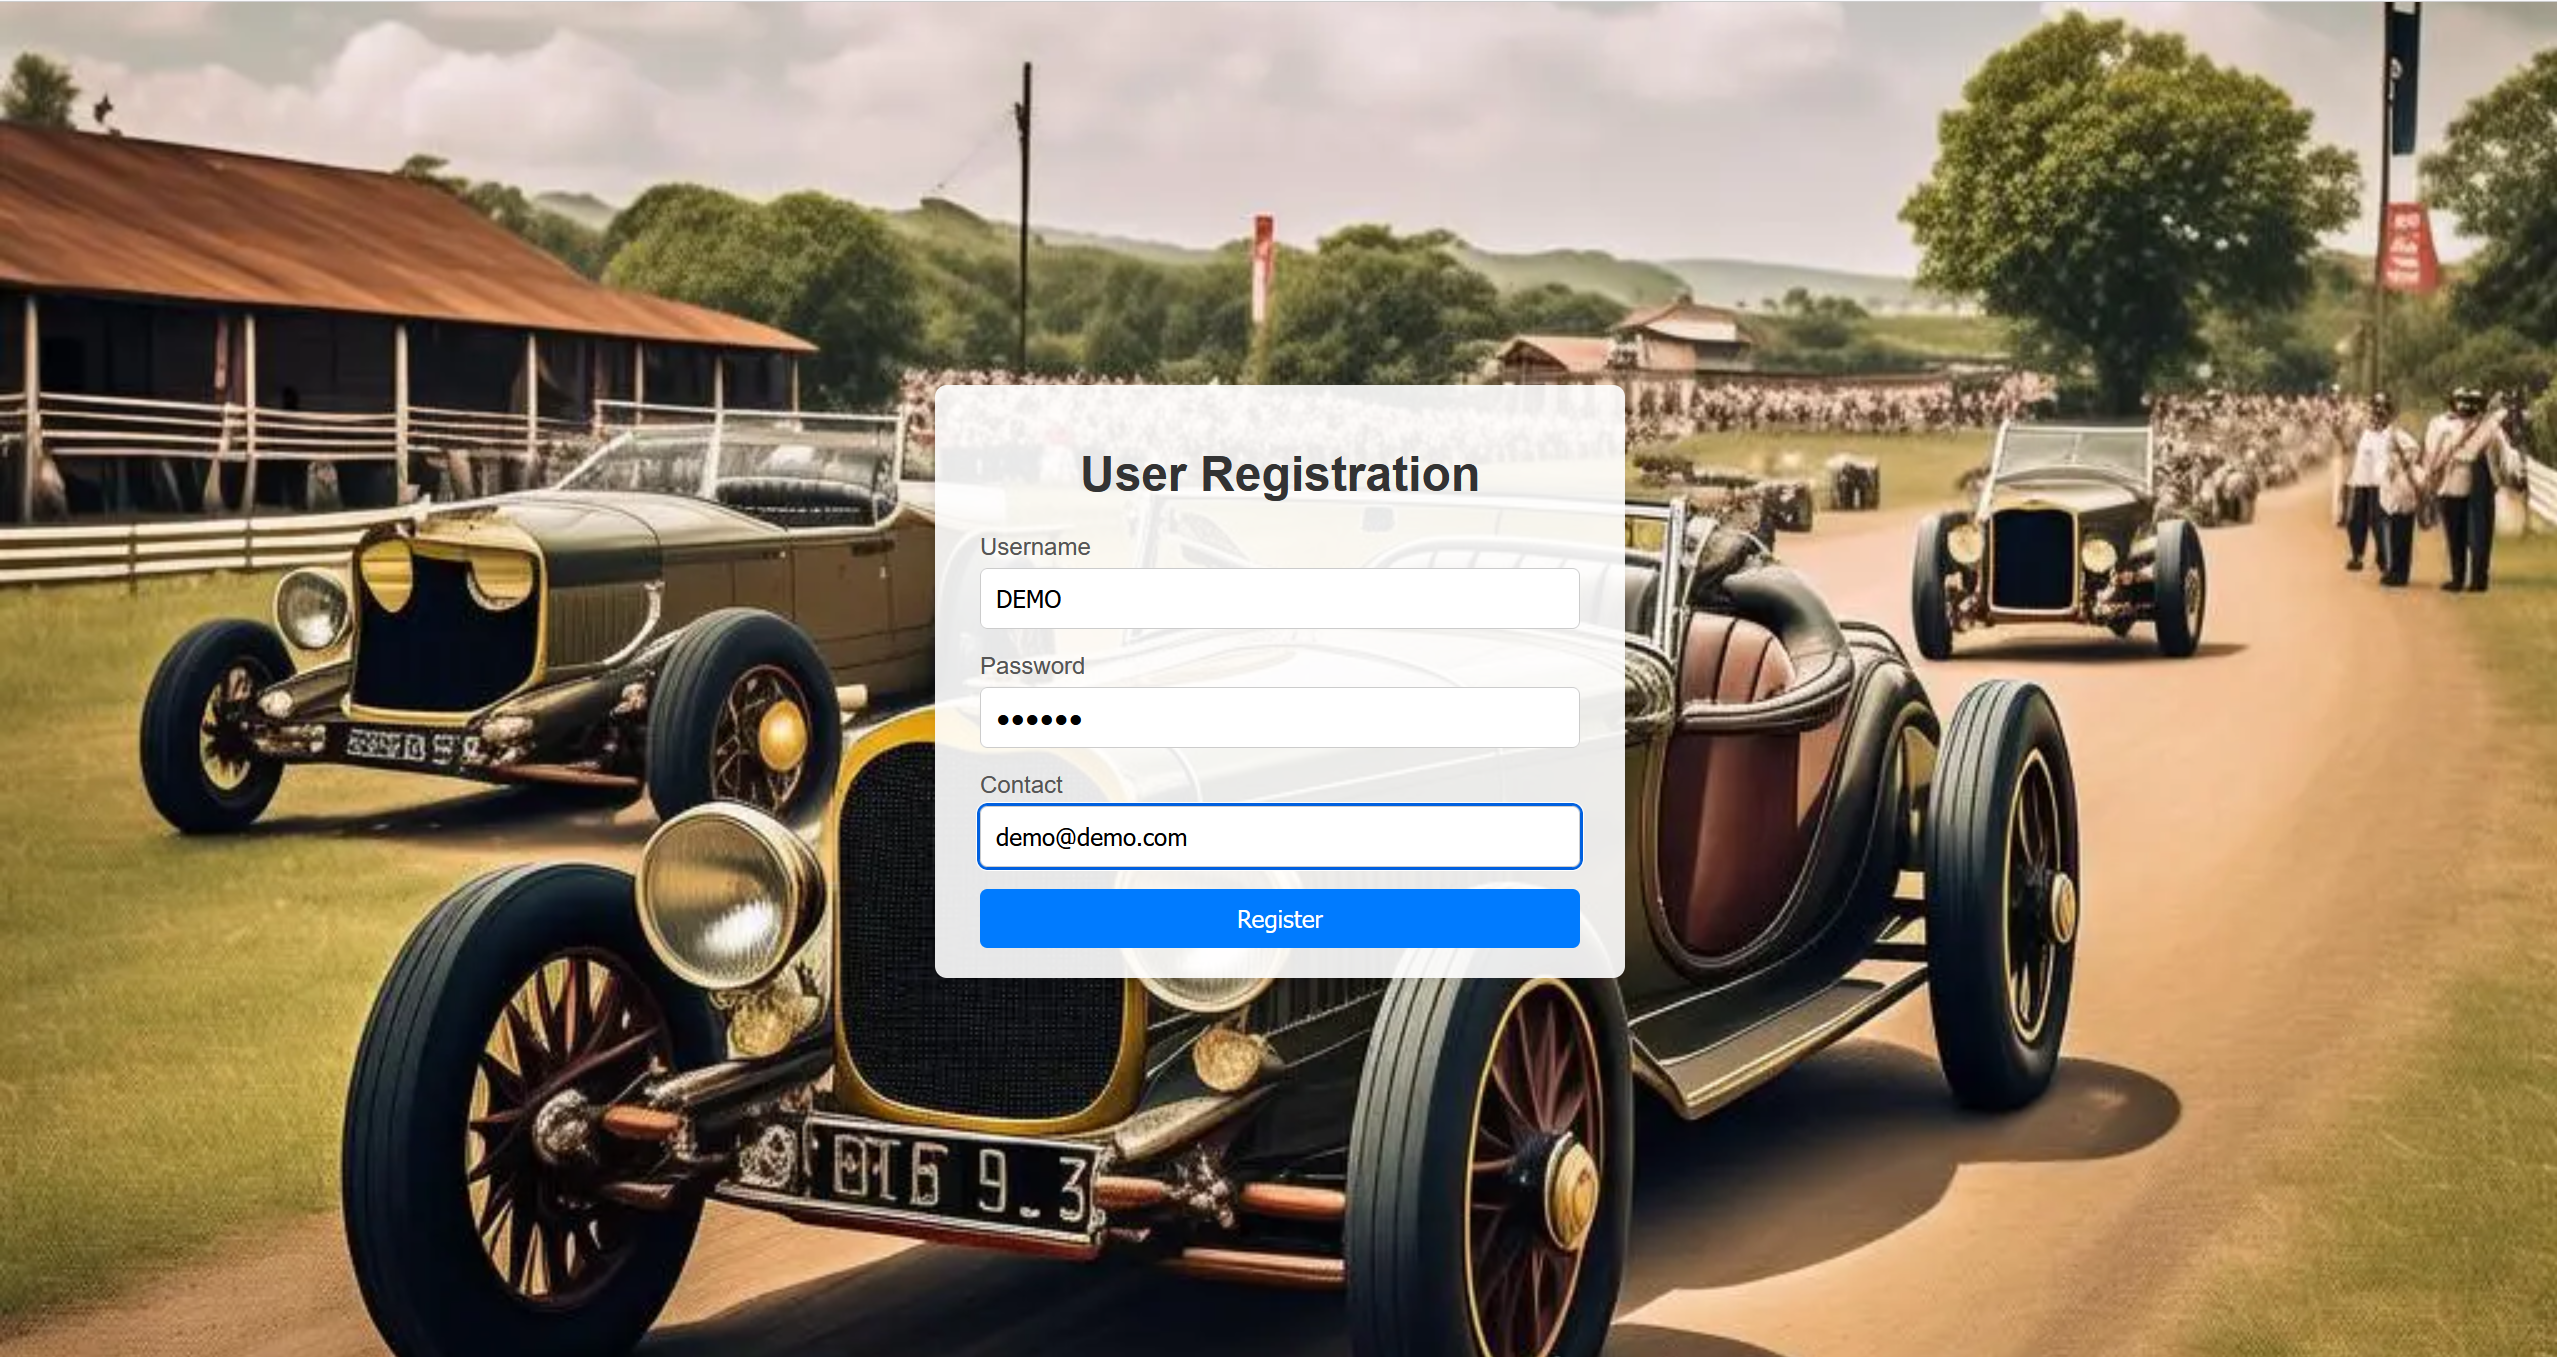
\includegraphics[width=0.8\textwidth]{pic/reg.png}
    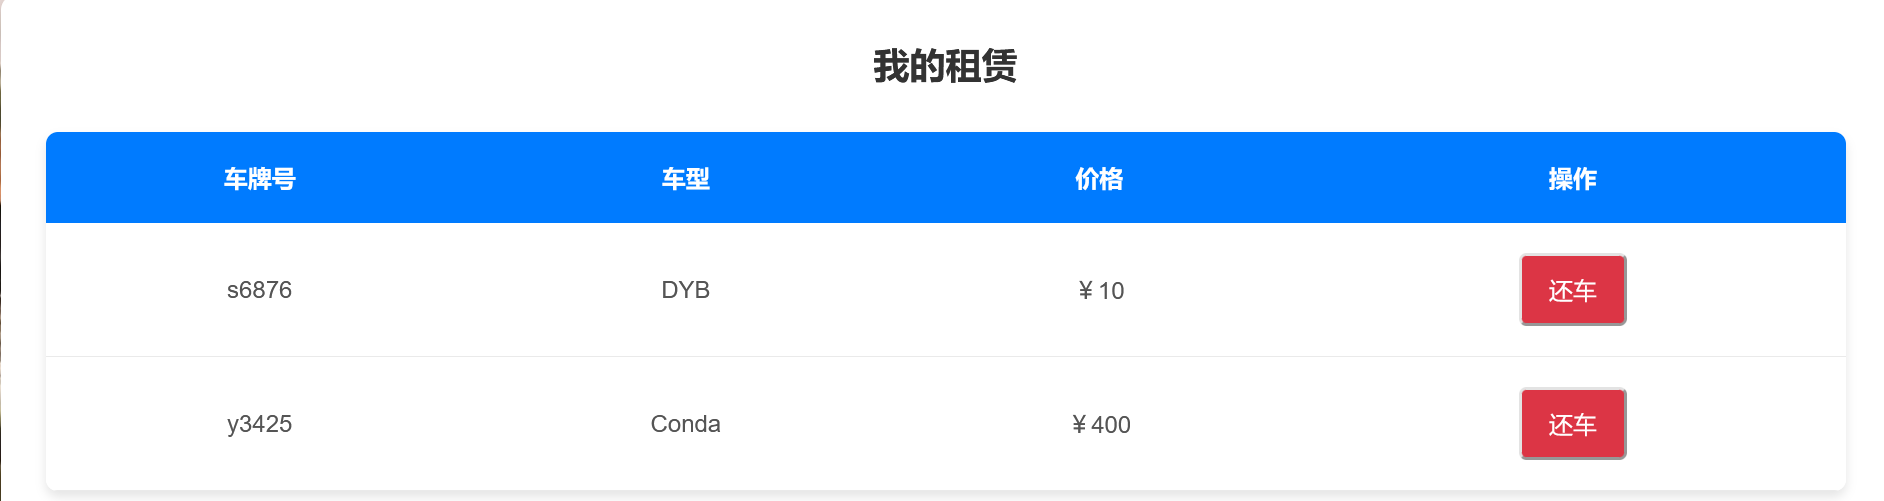
\includegraphics[width=0.8\textwidth]{pic/rent.png}
    \caption{用户租车信息列表}  % 图片标题
    \label{fig:rent}  % 图片标签,便于引用
\end{figure}
然后,用户通过点击还车键即可一键还车。换车后该车辆信息会从主页中移除,如图~\ref{fig:afrent}所示。
\begin{figure}[htbp]  % figure 环境用于插入图片并进行浮动
    \centering  % 图片居中
    % 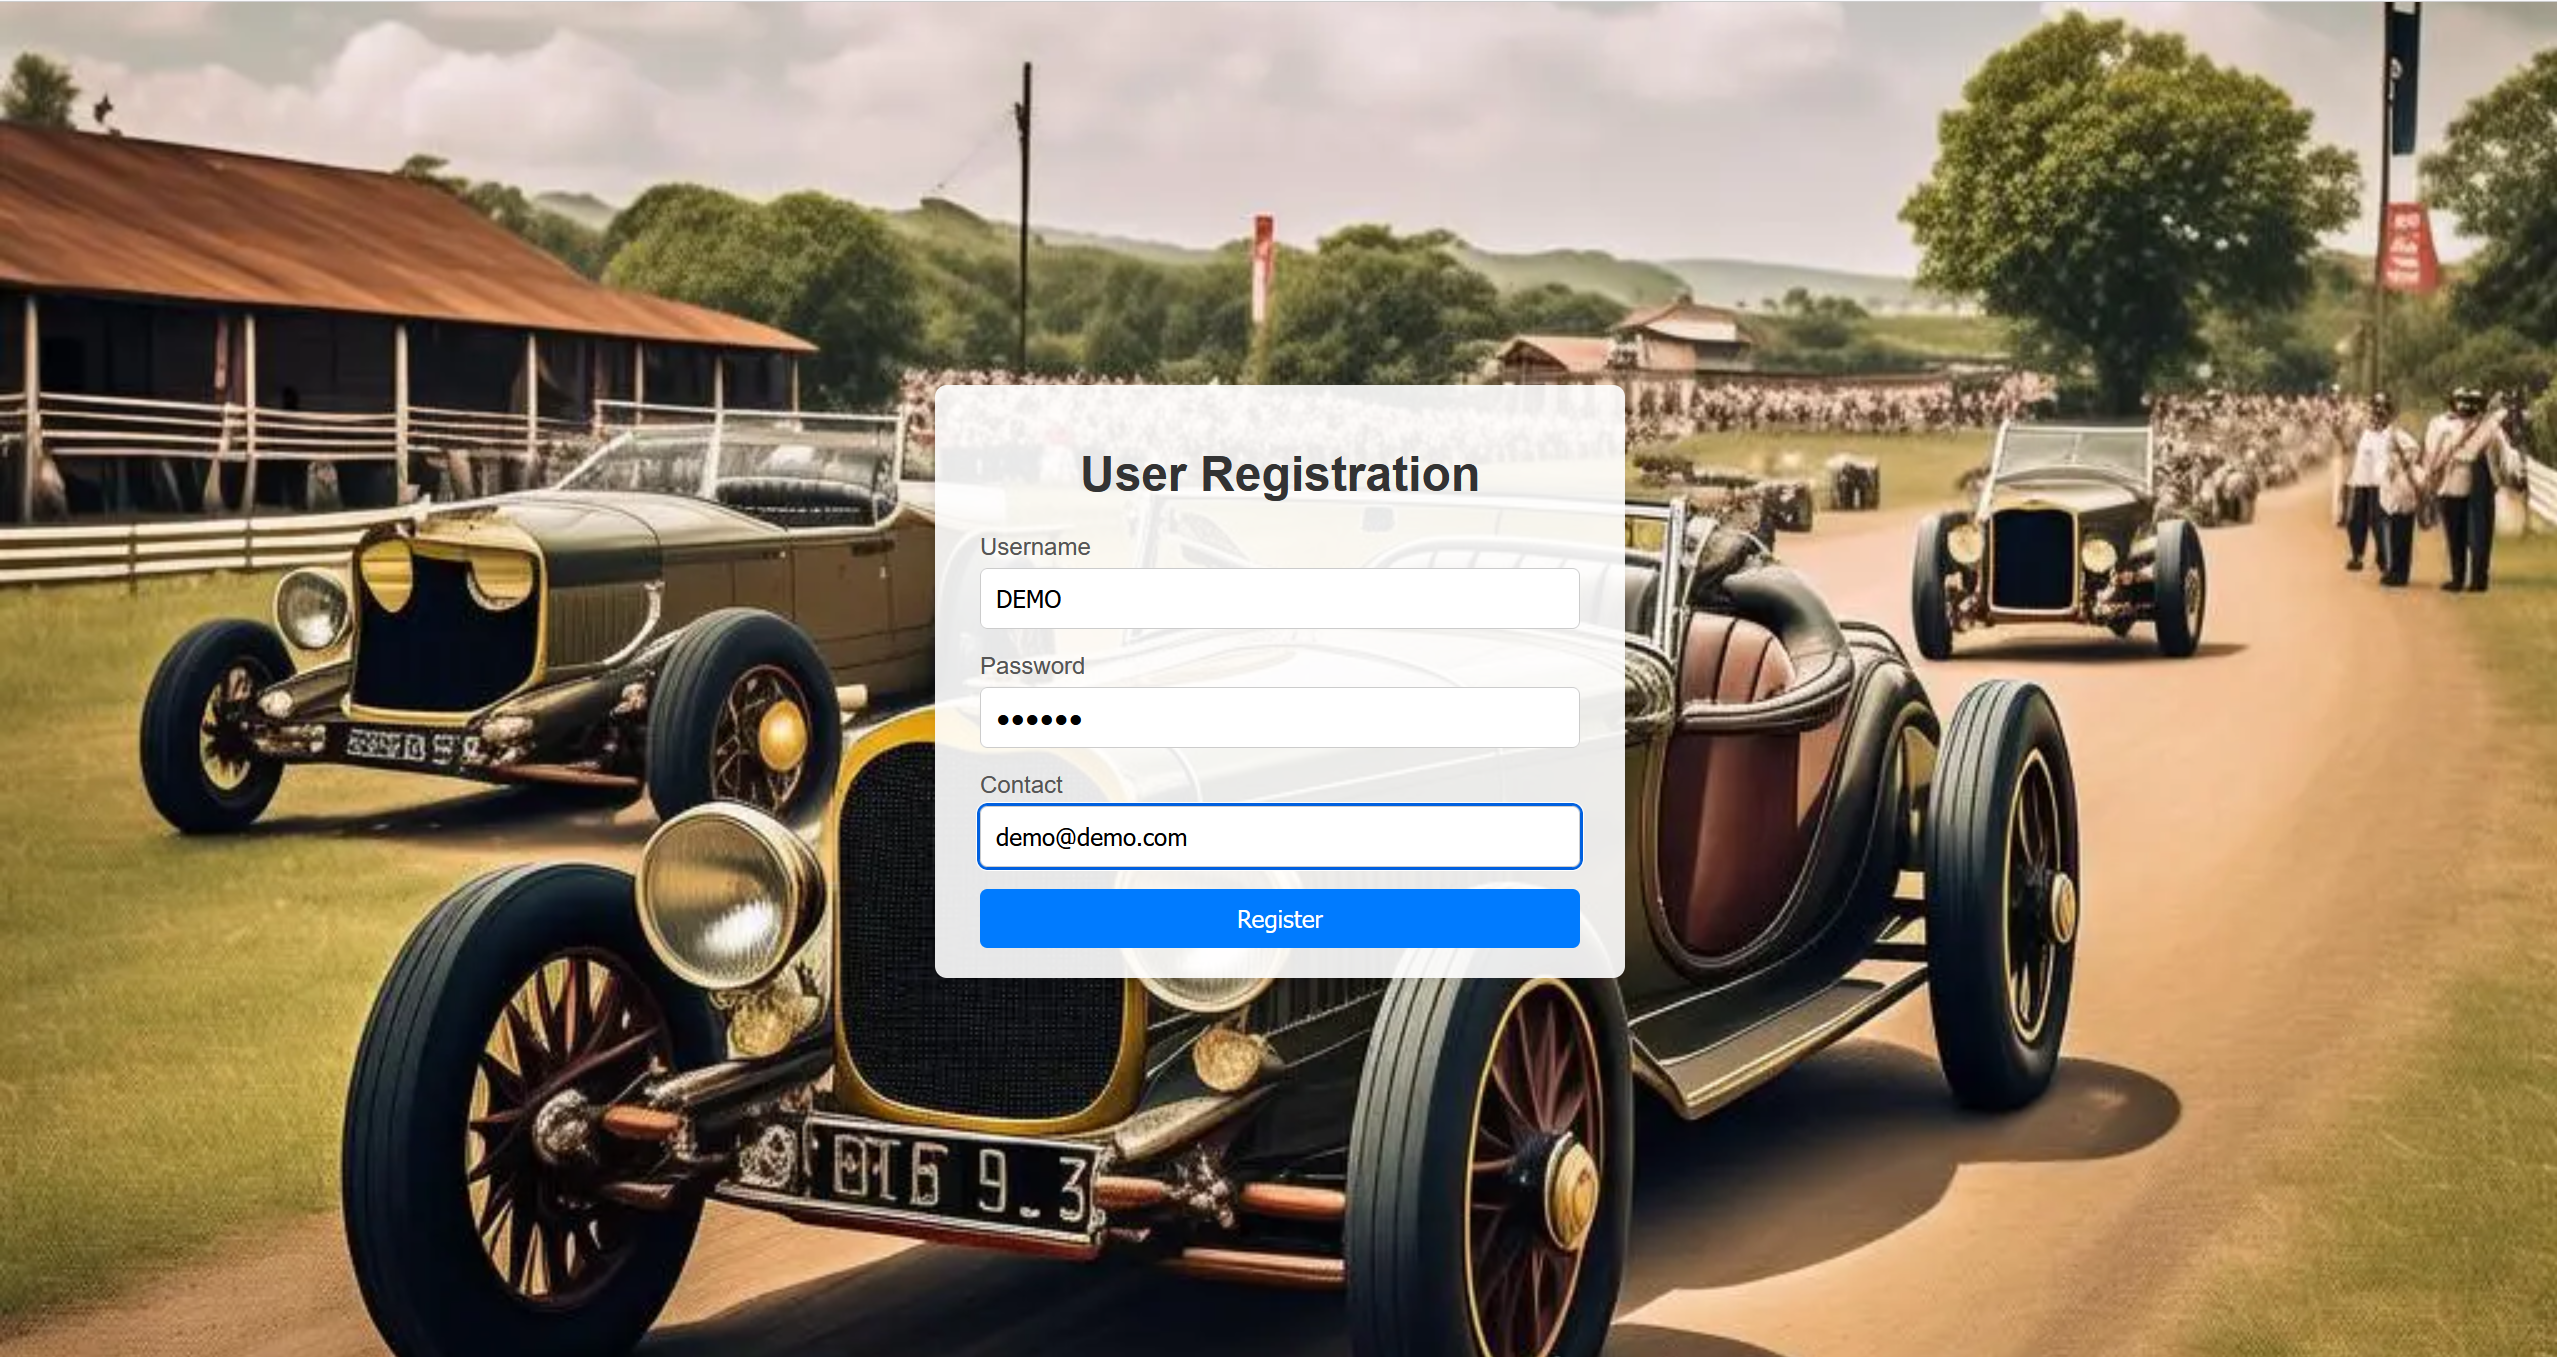
\includegraphics[width=0.8\textwidth]{pic/reg.png}
    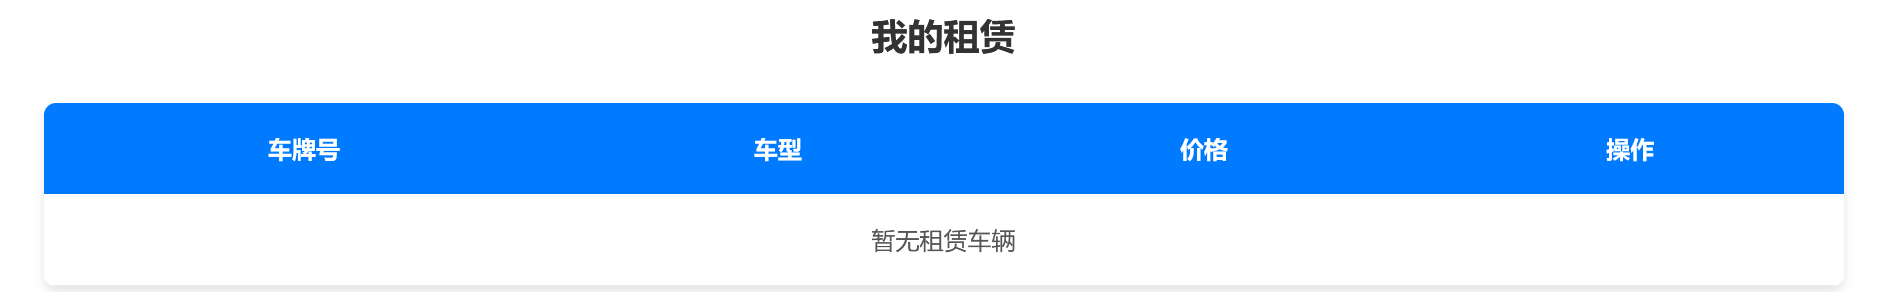
\includegraphics[width=0.8\textwidth]{pic/afrent.png}
    \caption{用户还车后列表信息}  % 图片标题
    \label{fig:afrent}  % 图片标签,便于引用
\end{figure}

\subsubsection{租车查询}
用户可以通过点击侧栏租车按键,查看车辆品牌信息,如图~\ref{fig:br}所示。
\begin{figure}[htbp]  % figure 环境用于插入图片并进行浮动
    \centering  % 图片居中
    % 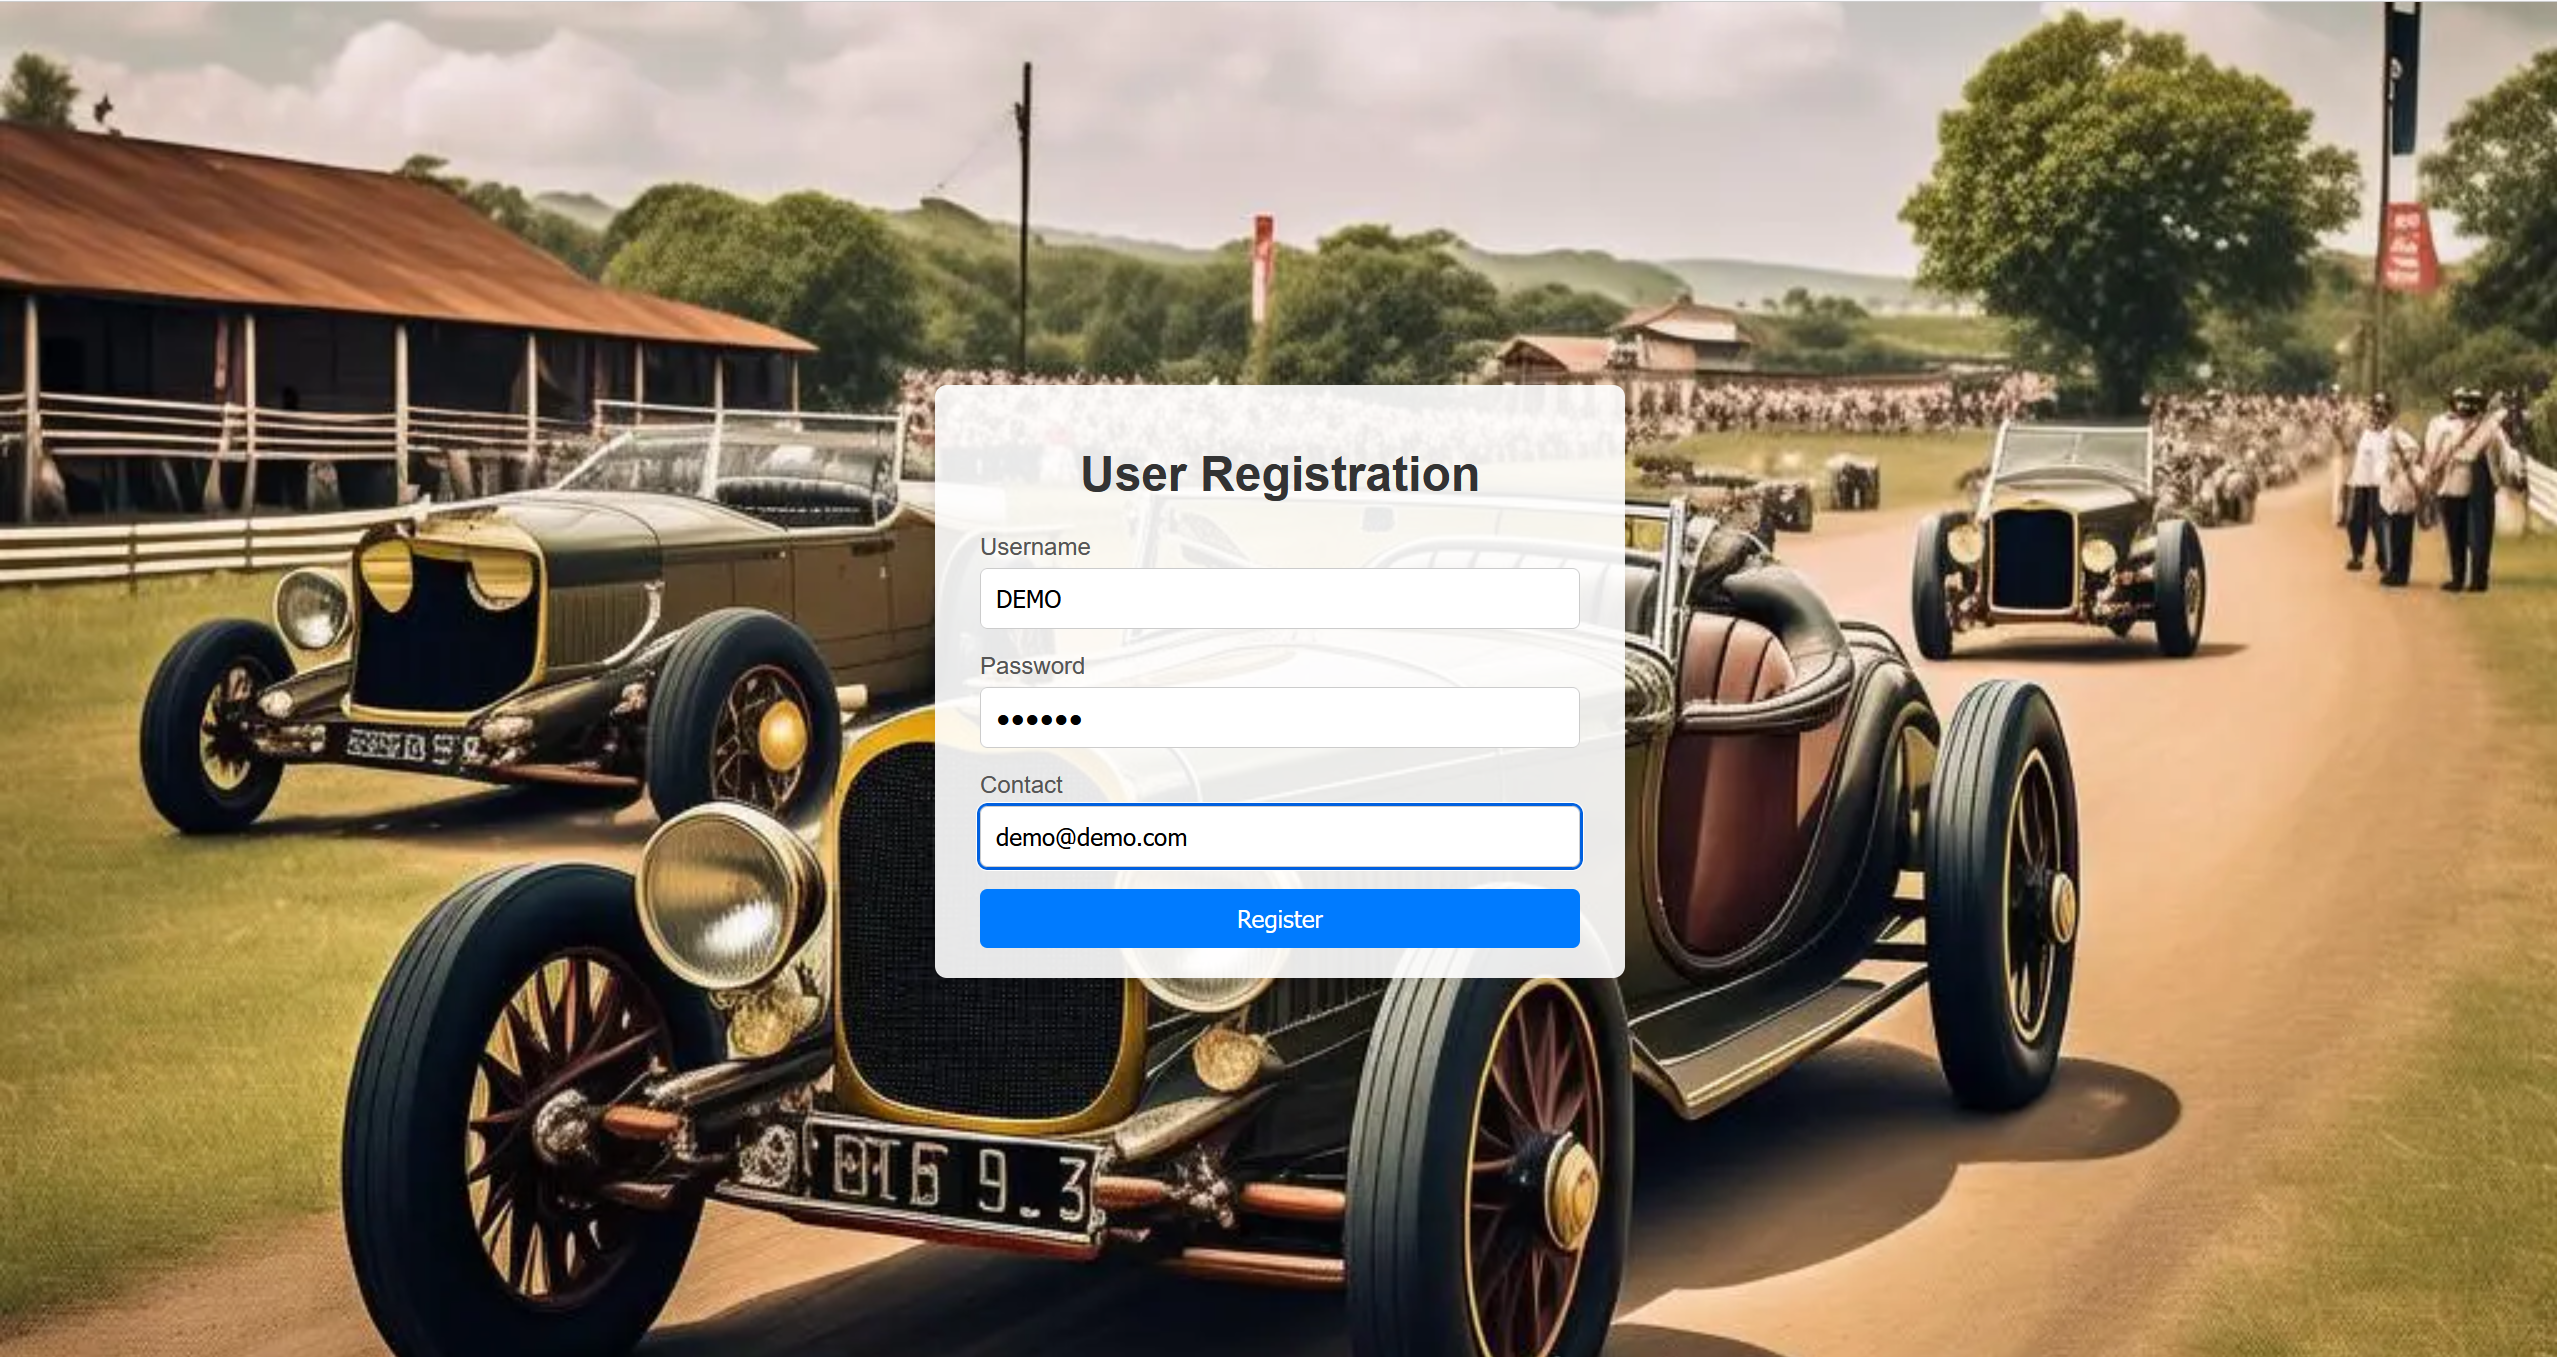
\includegraphics[width=0.8\textwidth]{pic/reg.png}
    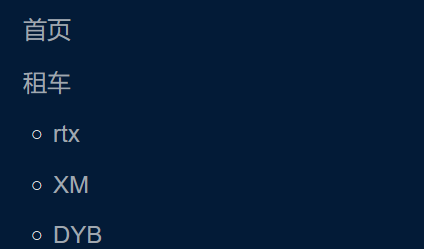
\includegraphics[width=0.8\textwidth]{pic/br.png}
    \caption{侧栏车辆品牌信息}  % 图片标题
    \label{fig:br}  % 图片标签,便于引用
\end{figure}
进一步的,用户可以点击自己感兴趣的车辆品牌,此时交互页面会跳转到含有该品牌车辆详细信息的界面供用户查看,如图~\ref{fig:car}所示。
\begin{figure}[htbp]  % figure 环境用于插入图片并进行浮动
    \centering  % 图片居中
    % 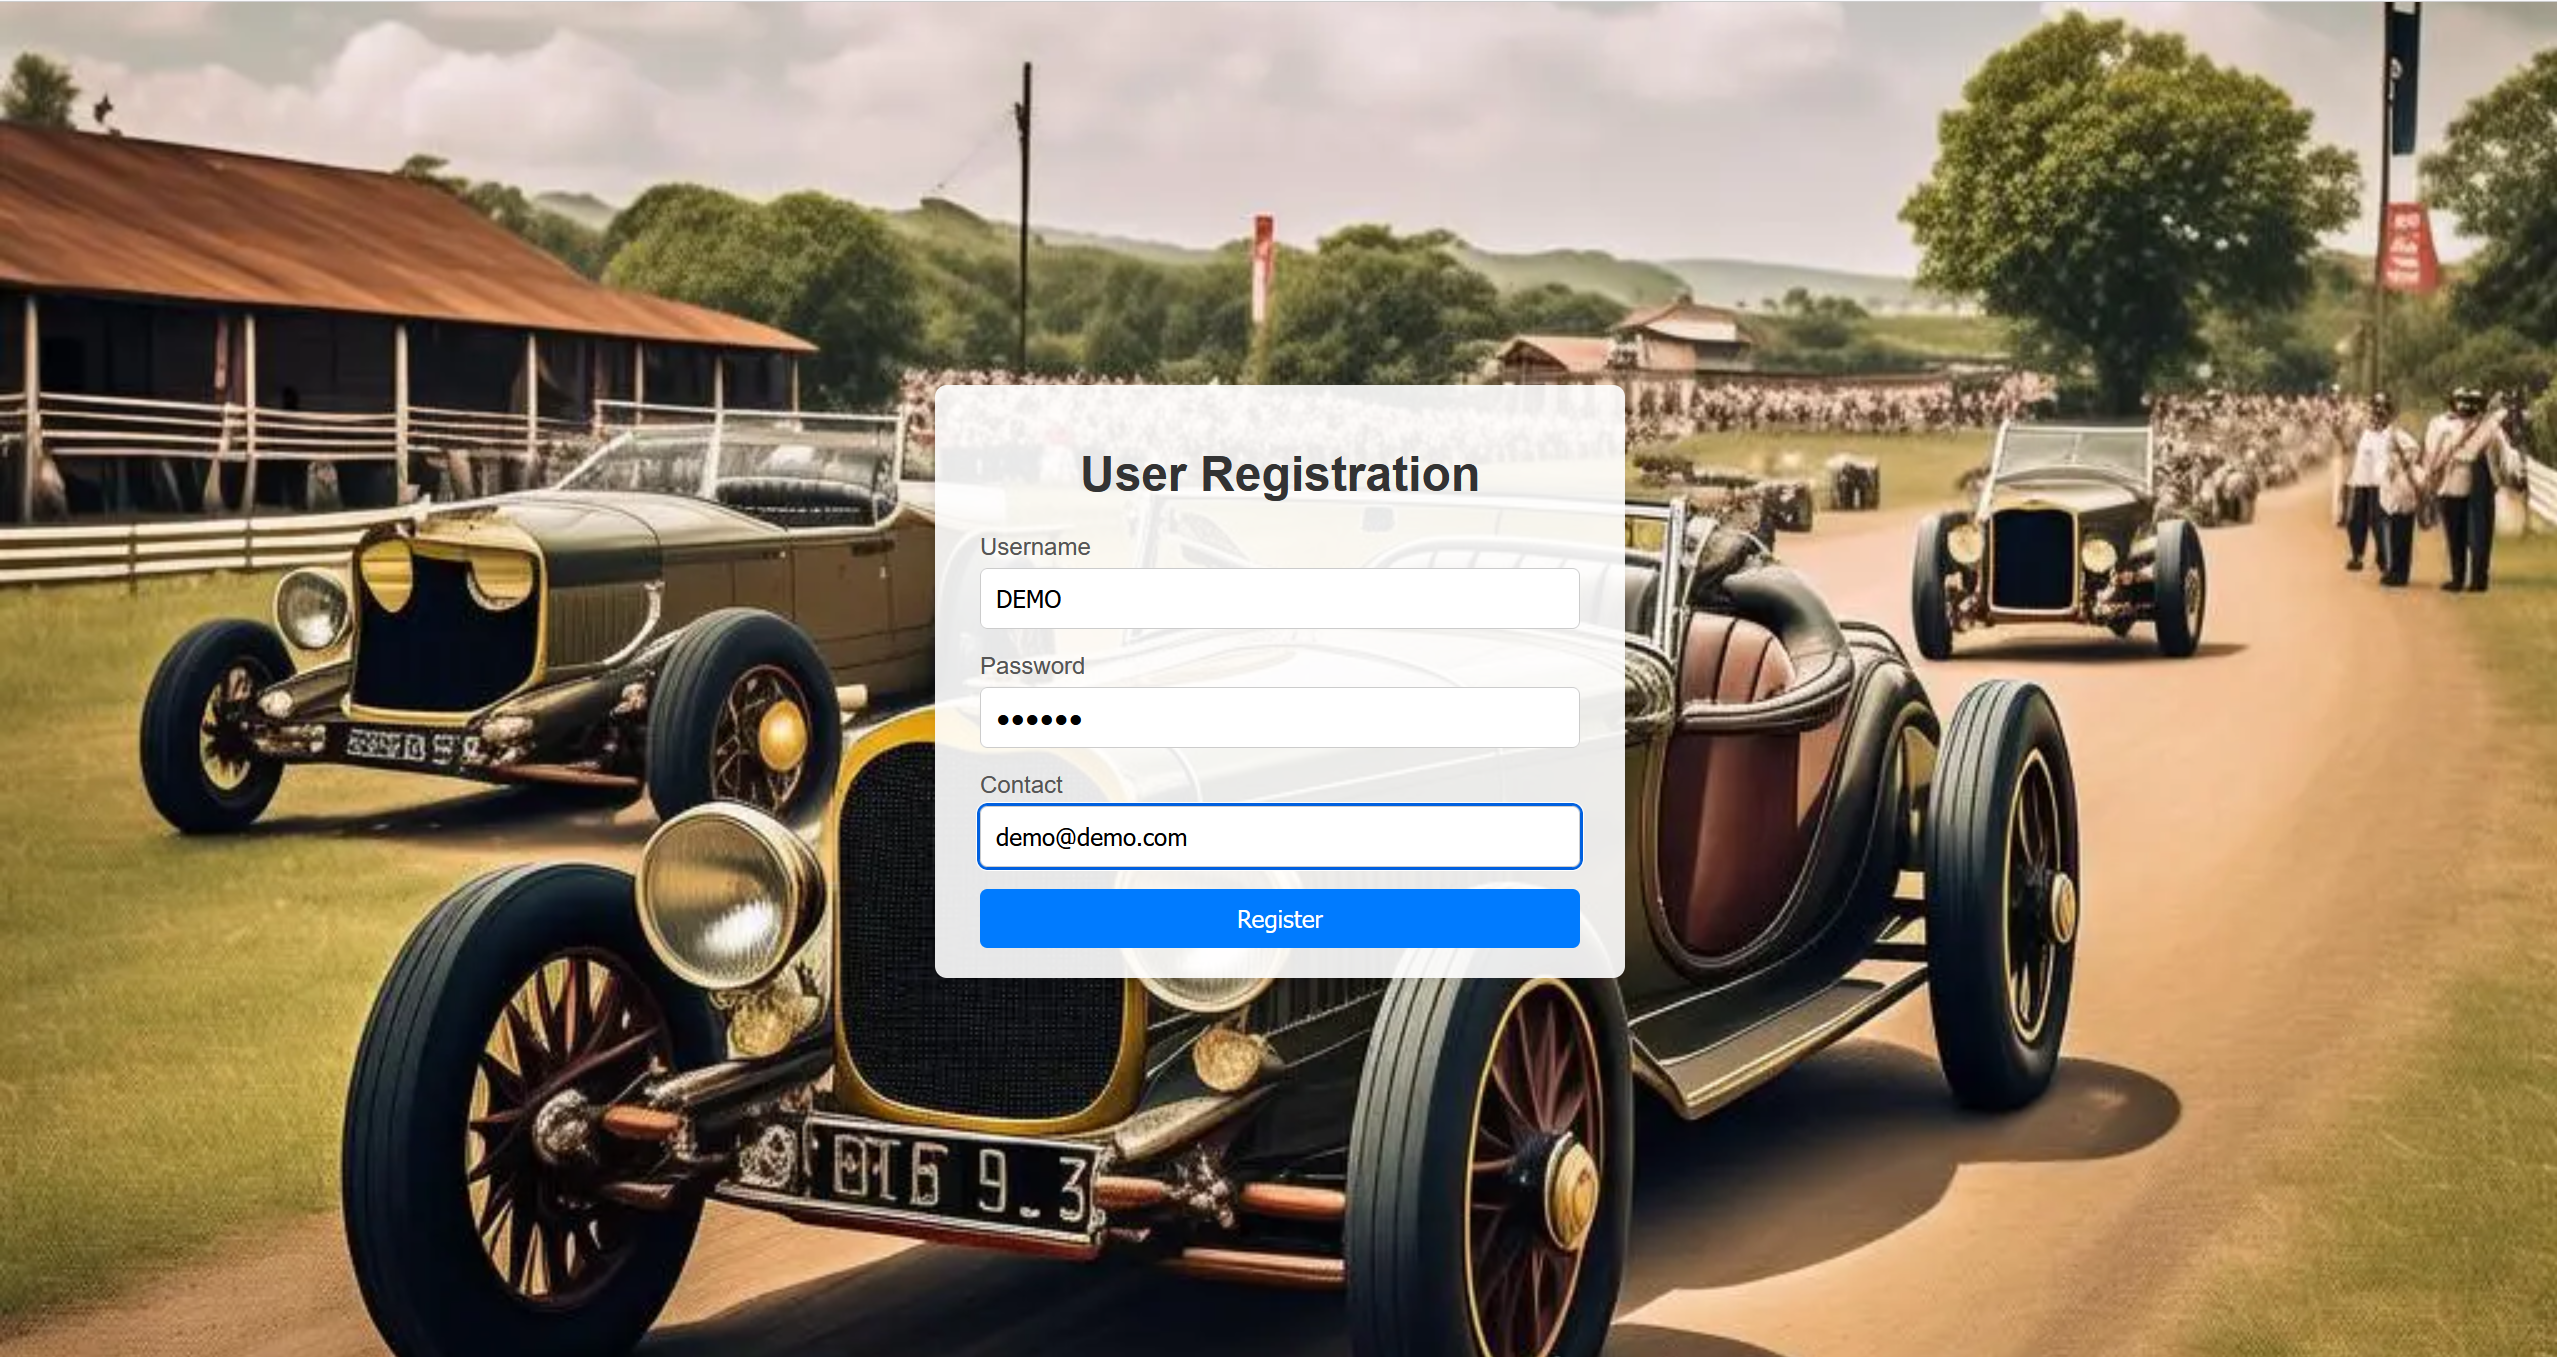
\includegraphics[width=0.8\textwidth]{pic/reg.png}
    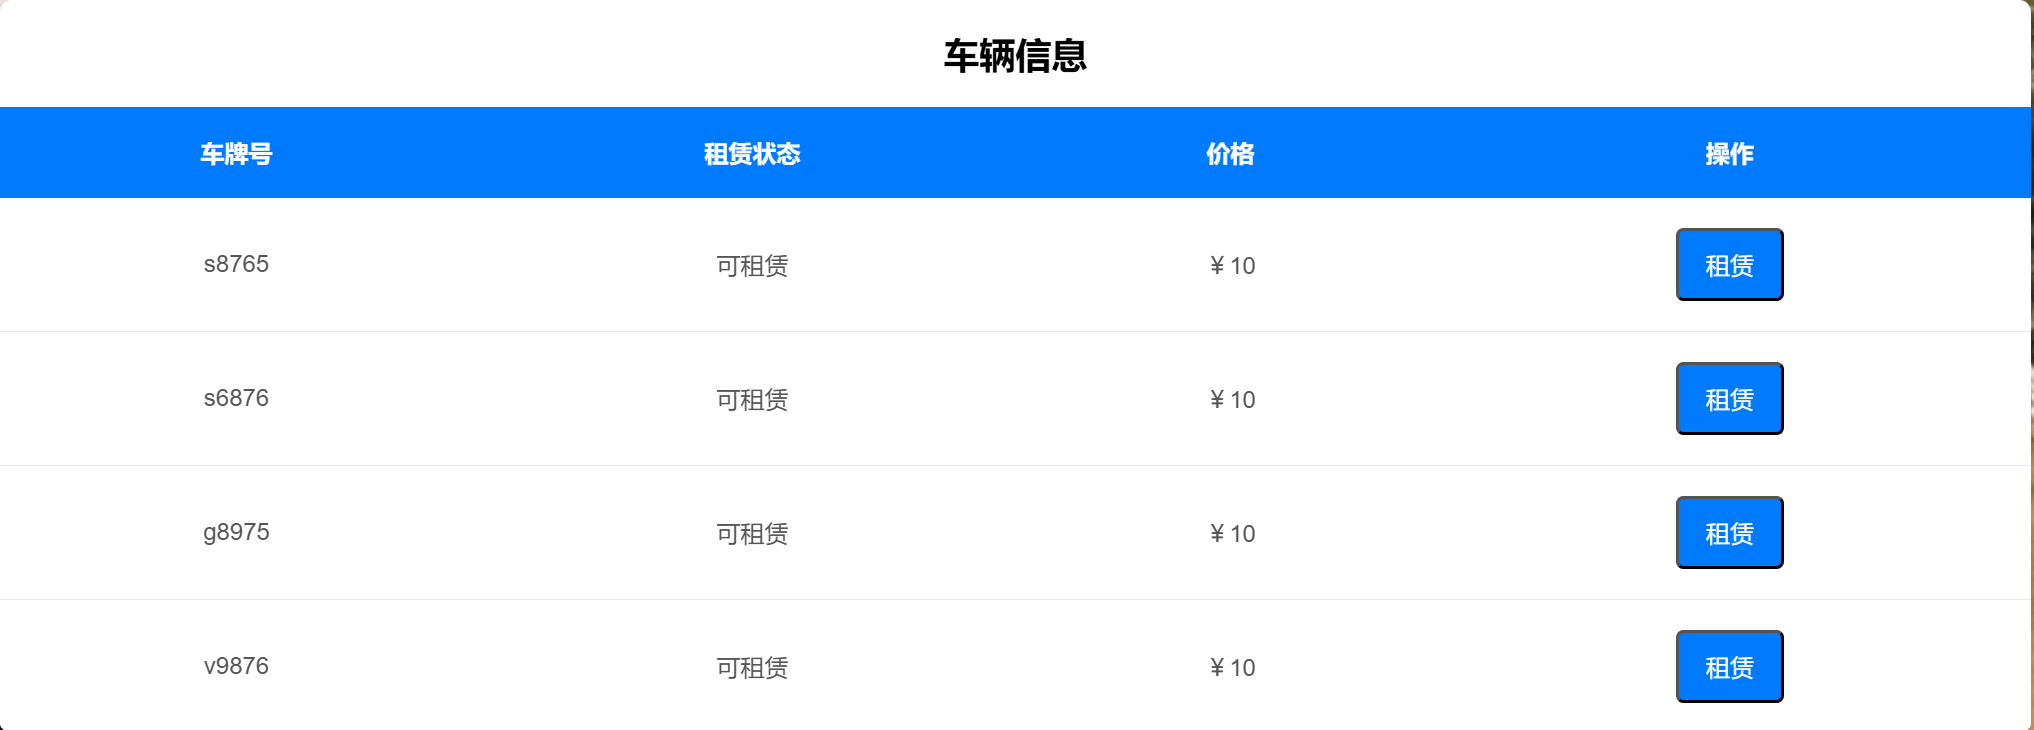
\includegraphics[width=0.8\textwidth]{pic/car.png}
    \caption{详细车辆信息}  % 图片标题
    \label{fig:car}  % 图片标签,便于引用
\end{figure}
对于想租的车辆,用户可以点击相应的租赁按钮进行租赁。当租赁成功后,页面会更新车辆状态,原按键变灰暂时不可用,如图~\ref{fig:rented}所示。
\begin{figure}[htbp]  % figure 环境用于插入图片并进行浮动
    \centering  % 图片居中
    % 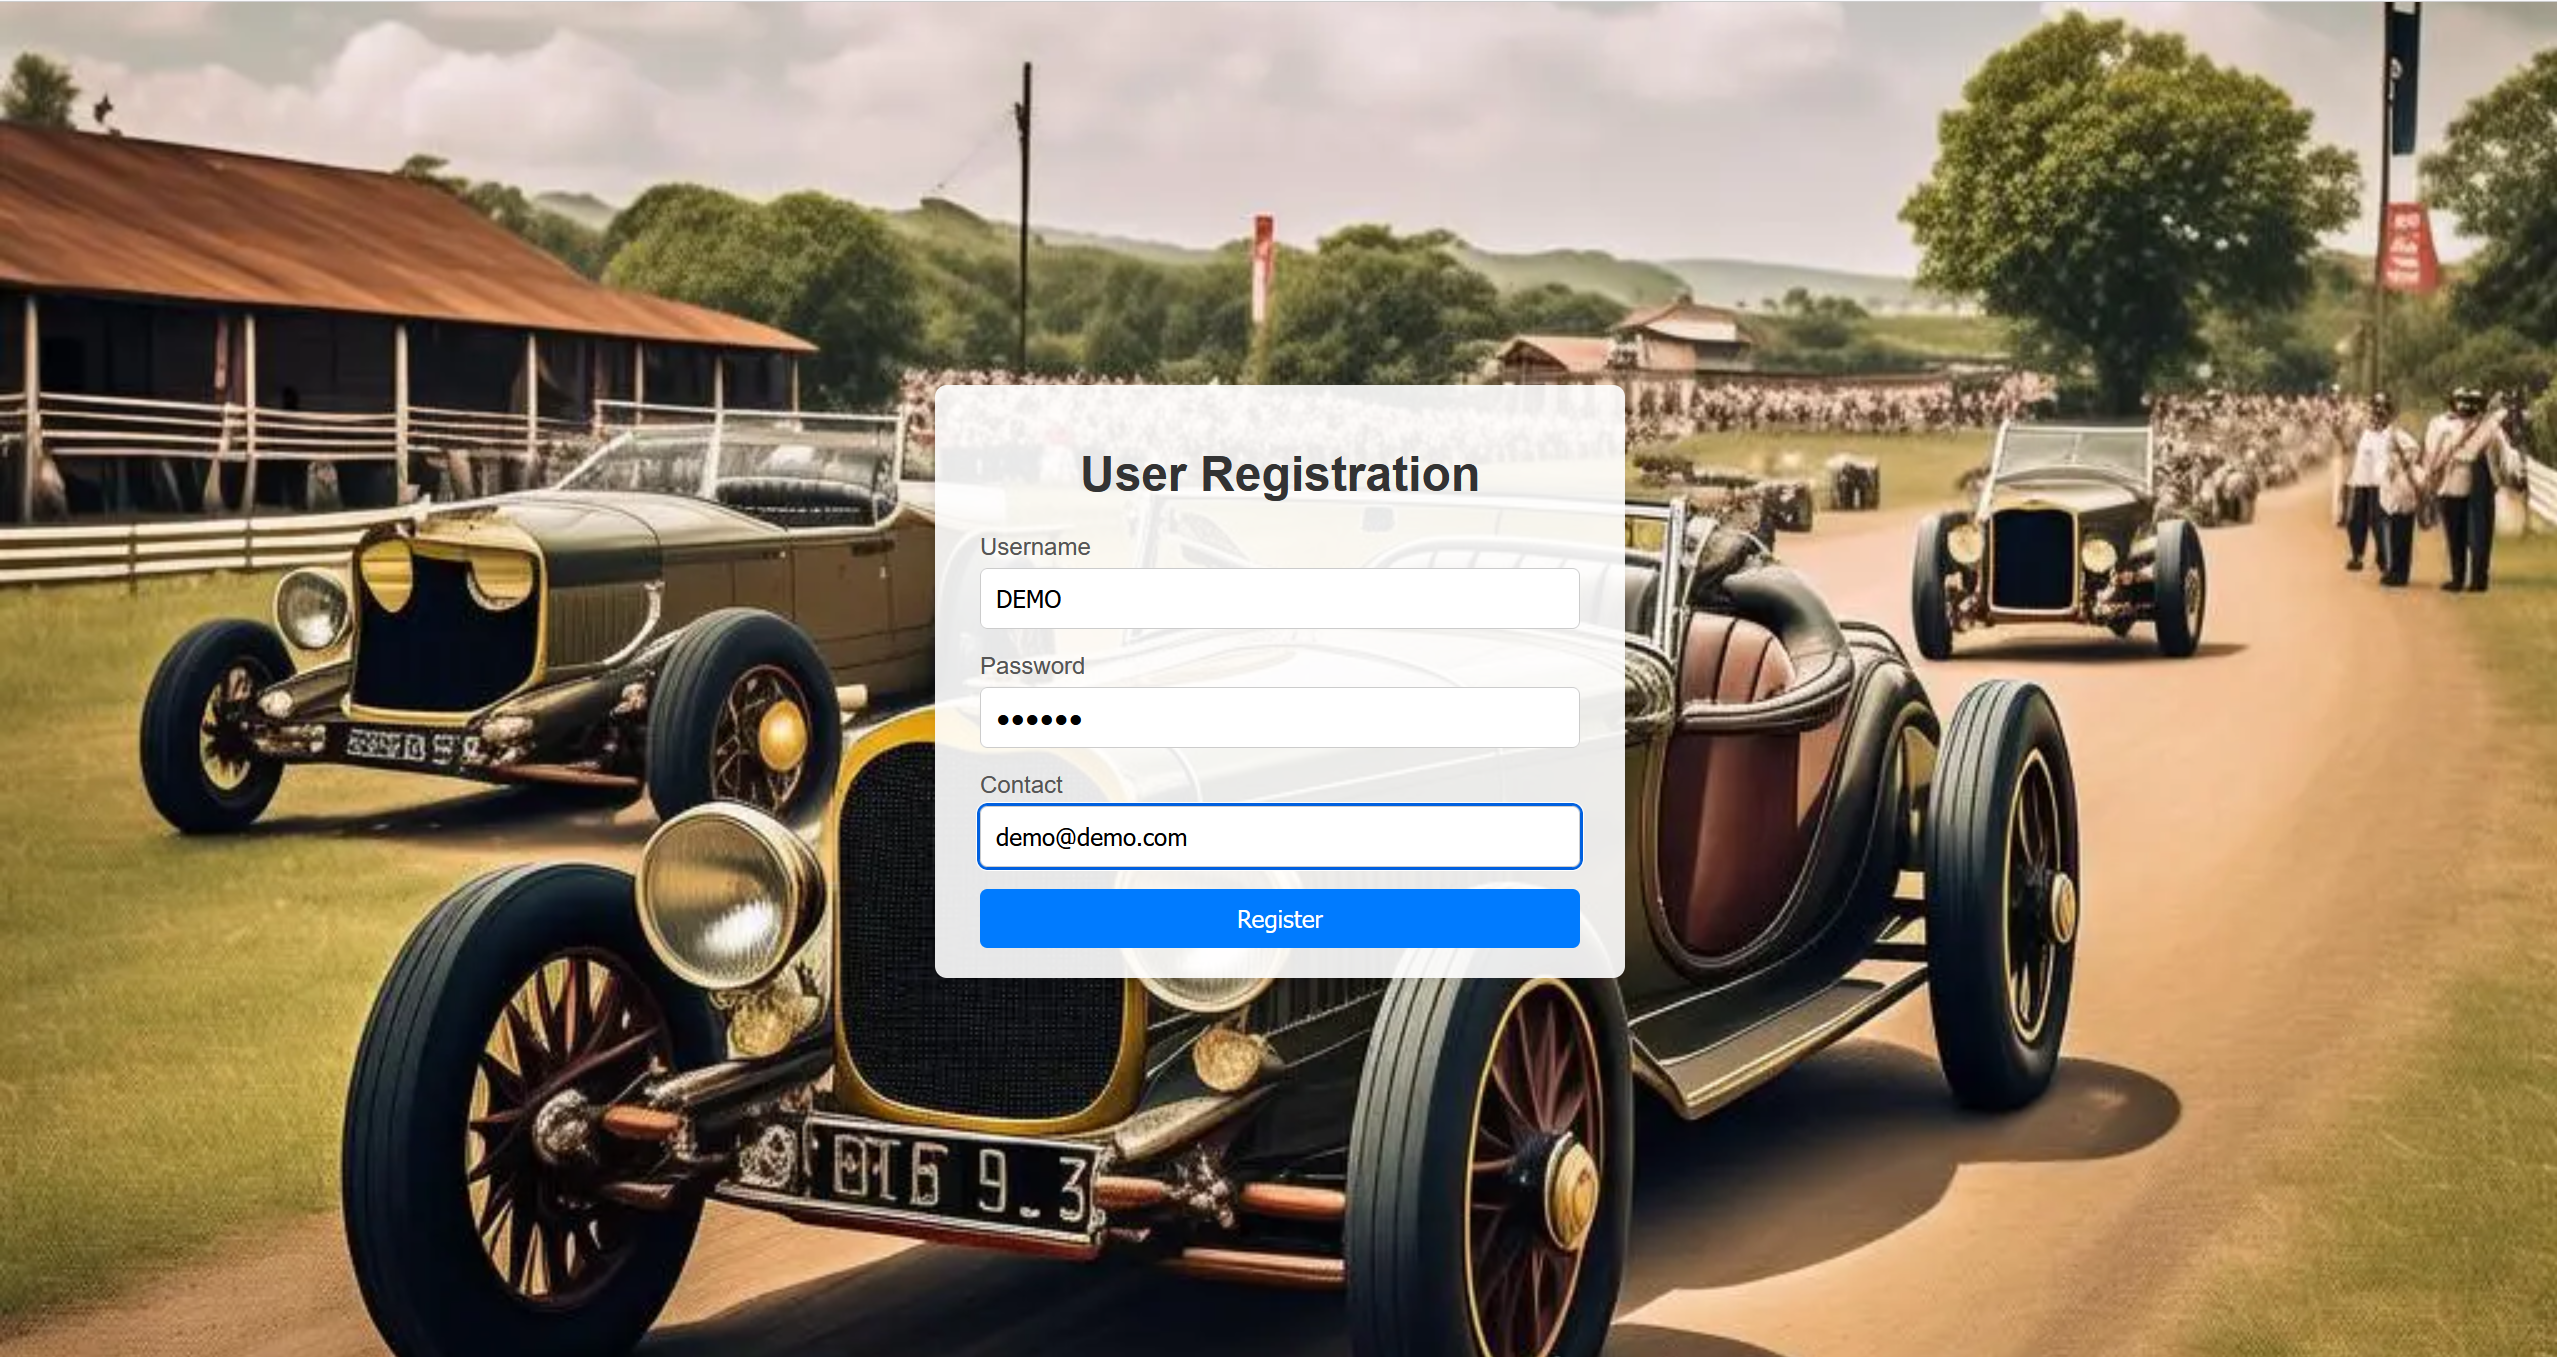
\includegraphics[width=0.8\textwidth]{pic/reg.png}
    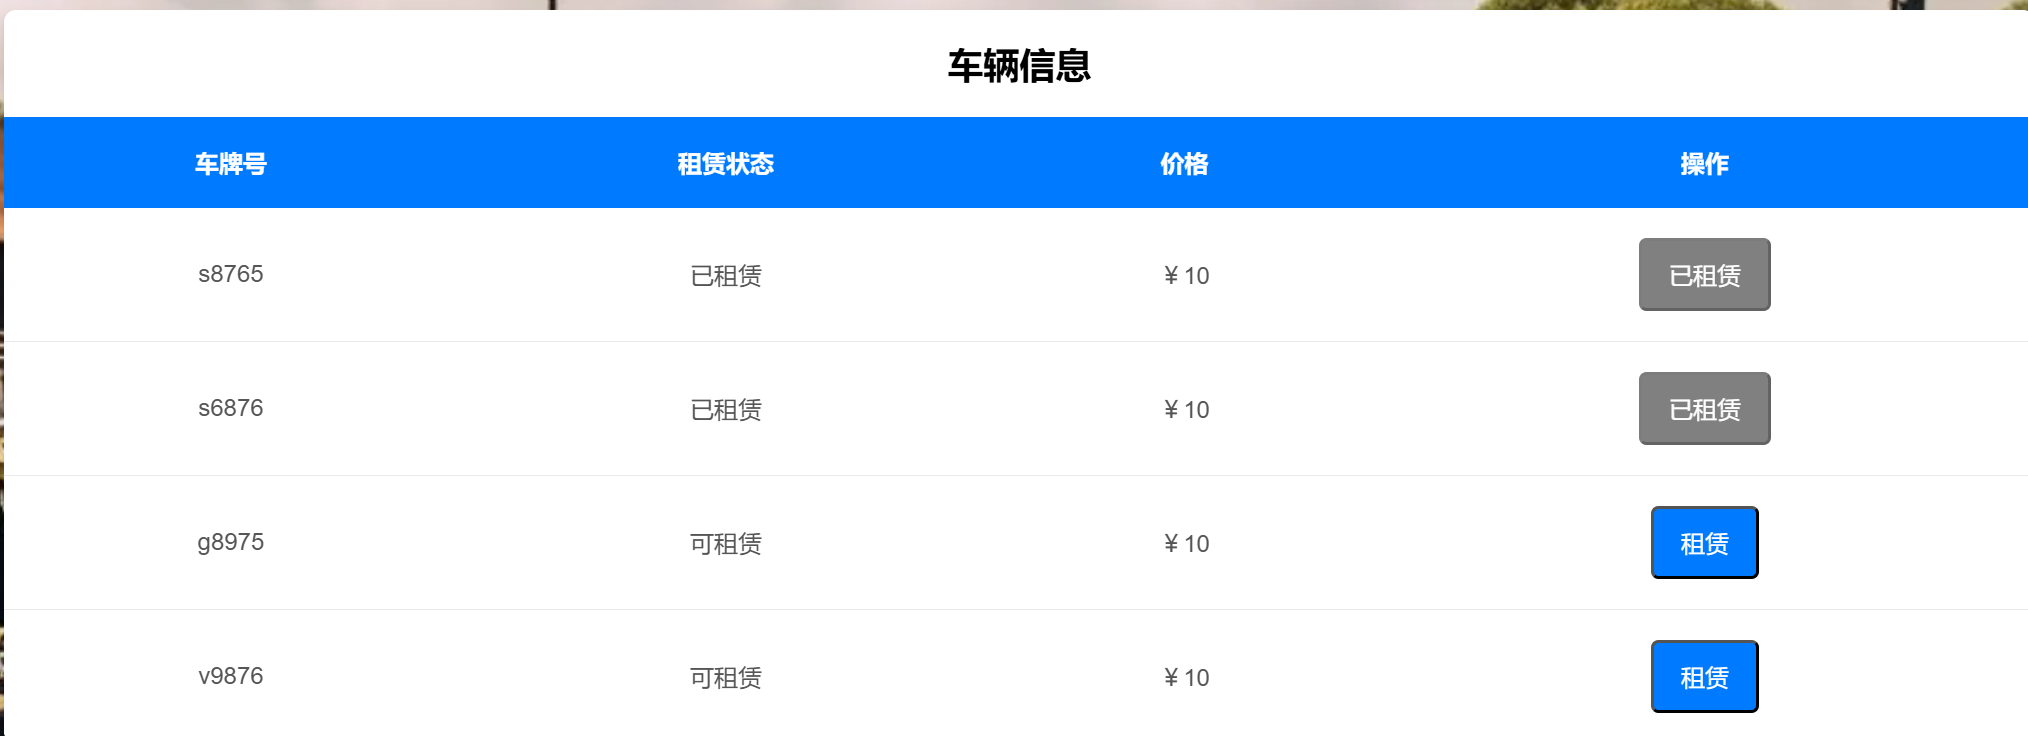
\includegraphics[width=0.8\textwidth]{pic/rented.png}
    \caption{详细车辆信息}  % 图片标题
    \label{fig:rented}  % 图片标签,便于引用
\end{figure}

\section{总结}

本实验设计旨在通过分析需求、设计系统架构和数据库结构,
开发一个功能完整的车辆租赁管理系统。设计过程中,
首先明确了系统所需实现的核心功能,
包括车辆信息管理、租赁管理、客户管理及系统安全等,并结合实际需求制定了详细的功能模块划分和技术架构。
系统架构上,采用了前后端交互的设计模式,
前端采用HTML和CSS等技术进行界面设计,
后端则基于Django框架处理数据逻辑及业务流程,
数据库部分使用了PostgreSQL以保证系统的数据安全性和一致性。
数据库设计遵循关系型数据库的设计规范,通过E-R图及关系模式分析,
合理设计了各数据表之间的关联关系,
并且通过标准化原则(如第三范式)保证了数据存储的高效性与无冗余性。

系统的开发过程中,后端逻辑层通过Django框架实现了用户管理、
车辆信息管理和租赁流程等功能模块,同时针对系统安全性进行了设计,
主要包括用户身份验证、数据加密、权限控制等措施,保障了系统的基本安全要求。
在前端设计上,注重界面的简洁性和用户操作的便捷性,通过直观的布局与交互设计,
确保了良好的用户体验。系统开发完成后,通过多轮功能测试和压力测试,
验证了各模块的稳定性与正确性,确保了系统的高效运行和良好的用户体验。

尽管系统已初步实现了预定功能目标,但在实际应用中,
仍存在一定的优化空间。在性能方面,数据库查询的效率有待提升,
尤其是在面对大量数据和高并发访问时,可以通过增加索引、优化SQL查询、
引入缓存机制等方式来优化响应时间和系统吞吐量。在系统架构方面,
未来可以考虑引入微服务架构,以便更好地应对系统扩展和高可用性要求。
此外,安全性方面,尽管基本采用了加密和权限控制,但还可以进一步完善,
如增加基于角色的访问控制(RBAC)、
引入多因素身份验证(MFA)等机制来增强系统的安全性。
功能层面,未来可通过引入数据分析模块,为系统提供数据驱动的决策支持,
例如租赁趋势分析、客户行为预测等,进一步提升系统的智能化水平。

综上所述,本实验设计实现了一个完整的车辆租赁管理系统,
涵盖了从需求分析到系统测试的全过程。
尽管系统具备了基本的功能和稳定的运行状态,
但在性能优化、安全增强和功能扩展等方面,
仍有较大的提升空间。未来可以通过持续优化架构设计、
引入新技术和完善系统功能,进一步提升系统的整体性能和用户体验。



\bibliography{custom}
\end{document}

